% Does Forgetting Help? -- JSS manuscript (single-file source; references in references.bib).
% All measured inference uses the frozen v12 runtime. Result tables are inlined from the
% outputs of scripts/analyze_completed_study.mjs (generated/*.tex); keep the two in sync.
\documentclass[a4paper,fleqn]{cas-sc}
\usepackage[T1]{fontenc}
\usepackage[authoryear,round]{natbib}
\usepackage{amsmath,amsfonts,amssymb,algorithm,algpseudocode,array,textcomp,url,graphicx}
\usepackage{tikz,pgfplots,listings,booktabs,xcolor,tcolorbox,seqsplit,needspace}
% Allow floats to share pages with following sections instead of forcing sparse pages.
\usepackage{placeins}
\hypersetup{hypertexnames=false,hidelinks}
\pgfplotsset{compat=1.17}
\usetikzlibrary{positioning,arrows.meta,fit,backgrounds,shapes.multipart,calc}
\tcbuselibrary{listings,skins}
\newcommand{\tool}{MORPH-FL}
\newcommand{\code}[1]{\texttt{\detokenize{#1}}}
\newcommand{\stereo}[1]{{\fontsize{6}{7}\selectfont\guillemotleft#1\guillemotright}}
\newcommand{\artifactpath}[1]{\nolinkurl{#1}}
\newcommand{\sourceid}[1]{\texttt{\seqsplit{#1}}}
\newcommand{\authoraction}[1]{\textbf{[AUTHOR TO PROVIDE: #1]}}
\lstset{basicstyle=\ttfamily\footnotesize,breaklines=true,columns=fullflexible,frame=single,numbers=left,numberstyle=\tiny,xleftmargin=1em}
\lstdefinestyle{morph}{language=Python,basicstyle=\ttfamily\normalsize,columns=fullflexible,keepspaces=true,keywordstyle=\color{blue!55!black}\bfseries,commentstyle=\color{black!55}\itshape,stringstyle=\color{orange!65!black},showstringspaces=false,numbers=none,frame=none,xleftmargin=0pt,aboveskip=0pt,belowskip=0pt}
\newtcolorbox{codebox}{enhanced,colback=black!5,colframe=black!22,boxrule=.4pt,arc=2mm,left=3mm,right=2mm,top=1.2mm,bottom=1.2mm}
% Compatibility for newer colortbl with pre-2024 array (no-op on current TeX).
\makeatletter
\providecommand\insert@pcolumn{\insert@column}
\providecommand\ext@lstlisting{lol}
\makeatother
% Allow large floats to share a text page and keep float-only pages well filled.
\renewcommand{\topfraction}{.95}
\renewcommand{\bottomfraction}{.85}
\renewcommand{\textfraction}{.05}
\renewcommand{\floatpagefraction}{.75}
\setcounter{topnumber}{3}
\setcounter{bottomnumber}{2}
\setcounter{totalnumber}{4}
\begin{document}
\let\WriteBookmarks\relax
\shorttitle{Does forgetting help in LLM fault localization?}
\shortauthors{Babaei}
\title[mode=title]{Does Forgetting Help? Studying Context Reset Policies in LLM Fault Localization}
\author[1]{Majid Babaei}[orcid=0000-0002-1394-4030]
\cormark[1]
\ead{majid.babaei@ufv.ca}
\affiliation[1]{organization={School of Computing, University of the Fraser Valley}}
\cortext[1]{Corresponding author.}

\begin{abstract}
Large language model (LLM) agents that localize faults from bug reports accumulate a dialogue in which checked facts, tentative explanations and the reasoning that links them are interleaved. When such an investigation stalls, a common remedy is to clear the context and start afresh, yet a reset that discards the dialogue can also discard what the agent has already established. We ask whether forgetting helps a localization agent, and what it should forget. We present MORPH-FL, a fault-localization framework for Python that keeps observations, hypotheses and dialogue in separate runtime models, so that a reset can clear dialogue and prune hypotheses while preserving every recorded observation. Using the framework as an experimental instrument, we compare four context policies on 50 SWE-bench issues from 12 repositories with two open 7B-scale code LLMs: adaptive reset on stagnation, continuous context, fixed-interval reset, and an observation-only view that shows the investigator its observations but neither its hypotheses nor its dialogue. Resetting the context, adaptively or on a schedule, did not change which issues were localized at rank one. The observation-only view localized more issues with one model and, with the other, kept grounded hypotheses on nearly every issue where the richer views kept almost none, at a higher time cost. Because rankings fall back to lexical retrieval when an investigation yields nothing, equal accuracy concealed very different investigations. The results suggest that what an agent is shown matters more than when its context is reset, and that context policies must be judged on investigation output and cost as well as accuracy.
\end{abstract}

\begin{keywords}
Fault localization \sep Large language models \sep Context management \sep Models at runtime \sep Empirical software engineering \sep Reproducibility
\end{keywords}
\maketitle
\raggedbottom

\section{Introduction}\label{sec:intro}
Anyone who has debugged a hard problem knows what it is like to be trapped by one's own reasoning. An early hunch decides which code gets read, which checks get run and how an ambiguous result is interpreted, and before long the investigation is circling. Stepping away and coming back with fresh eyes often helps. It helps, however, only because the developer keeps what was learned along the way, e.g., which files were ruled out. Effective forgetting is selective: \textit{it discards outdated assumptions while preserving relevant knowledge}.

LLM agents now carry out the same kind of investigation. Given a bug report and a repository, systems such as AutoFL, SoapFL and Agentless navigate the code, propose explanations and narrow the candidates until they can name the locations a developer should inspect~\citep{autofl2024,soapfl2025,agentless2025}. As the investigation proceeds, its context grows into a single transcript in which source facts, proposed fault mechanisms and the reasoning that connects them are interleaved. LLMs do not use such contexts reliably. Information in the middle of a long input is overlooked, irrelevant material distracts, and a model that takes a wrong turn early in a multi-turn conversation seldom recovers~\citep{lostmiddle2024,distract2023,multiturn2025,contextrot2025}. Agent designers respond by truncating, summarizing, masking or restarting the context~\citep{memgpt2024,sweagent2024,complexitytrap2025,forgetting2026}.

These remedies treat context as text to be shortened, and for fault localization that view misses what matters. A transcript contains information with different useful lifetimes. The observation that a given line of a fixed source revision contains a given expression remains true for the rest of the investigation. A hypothesis about why the failure occurs is a conjecture, and it can anchor the agent long after it has stopped being useful. Truncation and summarization cannot tell the two apart. A reset intended to escape a bad hypothesis may erase the refutation that had ruled it out, and a summary may turn a conjecture into something that reads like a fact. Whether forgetting helps a localization agent therefore depends on \emph{what} is forgotten and \emph{when}. To our knowledge, this question has not been studied.

We study it with \tool{}, a fault-localization framework for Python repositories. Drawing on models at runtime~\citep{modelsruntime2009} and on hypothesis-driven debugging~\citep{zeller2009}, \tool{} keeps the state of an investigation in four linked runtime models that describe the reported behavior, the source structure, the competing hypotheses and the evidence, and it builds every LLM request as a view of these models. Because facts and conjectures are distinct model elements, retention can be specified per kind of knowledge. When a stagnation monitor detects that the investigation has stopped producing new observations, \tool{} clears the investigators' dialogues and prunes the hypotheses to a small portfolio chosen for score and diversity, while every observation and the cumulative budget survive. Keeping state outside the dialogue is not new in itself; what \tool{} contributes is a precise retention specification and an implementation of it. The same machinery also lets us change what a request shows while holding everything else fixed, which makes \tool{} an instrument for comparing context policies as well as a localization approach.

We use this instrument to compare four context policies that span the space between never forgetting and forgetting everything except the facts. \emph{Continuous context} keeps all dialogue and hypotheses. \emph{Adaptive reset}, the full \tool{} design, resets when the monitor detects stagnation. \emph{Fixed reset} applies the same reset on a fixed schedule. The \emph{observation-only view} shows the investigator the report, source excerpts and recorded observations, but neither its earlier hypotheses nor its dialogue. We run every policy on the same 50 issues, drawn from twelve repositories of SWE-bench Lite and Verified~\citep{swebench2024,swebenchverified2024}, with two open code LLMs, Qwen2.5-Coder-7B and DeepSeek-Coder-6.7B. The study comprises all 400 model--workflow--issue investigations and 100 deterministic retrieval controls, and it is guided by four research questions:
\begin{description}
\item[RQ1 (Ranking)] How do the context policies compare in how well they rank the files and functions changed by the fix, with each model and against retrieval alone?
\item[RQ2 (Reset exposure)] How often do adaptive and fixed resets actually occur, and do investigations that can reset localize more issues than continuous context?
\item[RQ3 (Resources)] What token and time costs accompany each policy under a common budget?
\item[RQ4 (Investigation output)] What do the final hypothesis pools and response diagnostics reveal that ranking accuracy does not?
\end{description}

The anticipated benefit of context resets was not observed at file rank one. Neither adaptive nor fixed resets localized a single additional issue at rank one: with both models, the two reset policies and continuous context hit exactly the same issues. The policy that forgot the most did best. With Qwen, the observation-only view raised file Top-1 accuracy from 42\% to 50\%; with DeepSeek, it left accuracy unchanged but ended with grounded hypotheses on 47 of 50 issues, where the richer views ended with them on six or seven. This second result exposes a measurement problem that goes beyond our system. When no hypothesis survives, \tool{} falls back to lexical retrieval order, so the four DeepSeek workflows reached the same accuracy as retrieval alone while doing very different amounts of investigative work. The observation-only view was also 1.5 to 2 times slower. We treat it as a promising configuration to confirm rather than as a validated treatment, because we singled it out after seeing outcomes, it changes several parts of the request at once, and a known defect inflates the richer requests.

This paper makes four contributions:
\begin{itemize}
\item An investigation-state architecture that gives observations, conjectures and dialogue separate lifetimes, with source provenance, scoped assessments and an explicit obligation to preserve observations across a reset (Section~\ref{sec:approach}).
\item A complete, paired comparison of four context policies and two retrieval controls with two LLMs, which yields a negative result for stagnation-triggered resets and an exploratory positive result for an observation-only view (Sections~\ref{sec:study} and~\ref{sec:results}).
\item Evidence that ranking accuracy can conceal failed investigations behind a retrieval fallback, together with process measures---reset exposure, final-pool availability, response diagnostics and resource use---that expose such failures (Section~\ref{sec:rq4}).
\item A replication analysis that rebuilds every result table from the saved scores and checks the coverage of all study keys (Appendix~\ref{app:reproduction}).
\end{itemize}

The rest of the paper is organized as follows. Section~\ref{sec:background} defines the task and introduces a running example. Section~\ref{sec:approach} presents \tool{}. Section~\ref{sec:study} describes and justifies the study design, and Section~\ref{sec:results} reports its results. Section~\ref{sec:discussion} interprets them, Section~\ref{sec:threats} discusses threats to validity, Section~\ref{sec:related} relates our work to prior research, and Section~\ref{sec:conclusion} concludes.

\section{Background and Motivating Example}\label{sec:background}
\subsection{Report-Based Fault Localization}\label{sec:problem}
The input to report-based fault localization is a bug report and a snapshot of the repository before the fix. The output is a ranked list of source locations for a developer to inspect. We consider two granularities: files, identified by repository-relative paths, and functions, identified by qualified names within those files. A ranking says where to look; an explanation also says how an operation could cause the reported failure.

Evidence about an explanation comes from checks of different strength. A source check establishes that a line contains some text, an abstract syntax tree (AST) query establishes that a file contains a syntactic structure, and an execution procedure establishes what the program does for chosen inputs. Throughout the paper, a check \emph{supports} a hypothesis when the observed value equals the value its prediction expects, for example when a predicted expression is present in the inspected code. Support from a source or AST check is therefore a static fact; it does not show that the reported execution reached that code. The investigator sees the report, the pre-fix source and the procedures it is allowed to run. It never sees the reference patch, which the evaluation uses only to derive the target locations.

\subsection{Motivating Example}\label{sec:example}
Listing~\ref{lst:example} shows a constructed example that we use throughout the paper. A report states that setting \code{enabled} to false still displays a feature. The handler passes the normalized option to a rendering function, which is omitted. The fault is in \code{normalize}: the expression \code{options.get("enabled") or True} evaluates to true when the option is false. Line numbers are counted within each file, so the defaulting return is \code{config.py:2} and the handler's return is \code{handler.py:4}.

\begin{figure}[pos=H]
\refstepcounter{lstlisting}\label{lst:example}
{\centering\sffamily\footnotesize Listing~\thelstlisting. Constructed a configuration fault in two Python files.\par}
\vspace{3pt}
\begin{codebox}
\begin{lstlisting}[style=morph]
# config.py
def normalize(options):
    return {"enabled": options.get("enabled") or True}

# handler.py
from config import normalize
def handle(options):
    config = normalize(options)
    return render(config["enabled"])
\end{lstlisting}
\end{codebox}
\end{figure}

Because the report describes what is displayed, an investigator may well suspect the handler first. Two explanations then compete. The \emph{bypass} hypothesis claims that the handler renders the raw option instead of the normalized value; it predicts that the handler's return expression mentions \code{options}. The \emph{defaulting} hypothesis claims that \code{normalize} replaces an explicit false with a default; it predicts a return expression containing \code{or True}. Table~\ref{tab:example_checks} shows one AST check for each prediction. The first contradicts the bypass prediction and the second supports the defaulting prediction. Neither check executes the program, so the defaulting explanation remains a hypothesis, now with structural support.

\begin{table}[pos=!htbp]
\caption{Two AST checks on Listing~\ref{lst:example}.}\label{tab:example_checks}
\centering\small\setlength{\tabcolsep}{2pt}
\begin{tabular}{@{}>{\raggedright\arraybackslash}p{.17\columnwidth}>{\raggedright\arraybackslash}p{.46\columnwidth}>{\raggedright\arraybackslash}p{.10\columnwidth}>{\raggedright\arraybackslash}p{.19\columnwidth}@{}}\toprule
Hypothesis & AST query (expected result) & Result & Assessment\\\midrule
Bypass & A \code{return} in \code{handler.py} contains \code{options} (true) & False & Contradicts\\
Defaulting & A \code{return} in \code{config.py} contains \code{or True} (true) & True & Supports\\
\bottomrule\end{tabular}
\end{table}

Now suppose the investigation stalls and later rounds keep re-proposing the same two checks without learning anything new. Restarting with an empty context would force the investigator to rediscover both results. Keeping only the main explanation would also be a problem if observations were not stored separately. Evidence against the bypass idea could be lost in the next context, allowing the idea to return. The example thus captures the dilemma of forgetting in miniature. The old conversation should be removed, but the two observations must be kept. It is also unclear whether both explanations should remain visible. \tool{} was designed to make this choice explicit and to keep observations and a portfolio of competing explanations while clearing dialogue. This paper examines whether to show these explanations in future requests.

\subsection{Models at Runtime}\label{sec:mde_background}
To make such retention decisions explicit, \tool{} leverages model-driven engineering (MDE) techniques. In MDE, a model represents selected aspects of a system in an explicit structure. A metamodel defines the admissible element types, attributes and relationships, and transformations derive models or views from other models~\citep{mde2006}. Models do not have to be created at design-time. The models@run.time paradigm keeps a model of a running system and uses it to drive the system's adaptation~\citep{modelsruntime2009}, similar to the monitor, analyze, plan, and execute cycle in autonomic computing~\citep{mapek2003}. \tool{} applies this idea to an investigation rather than a deployed system. Its models describe what the investigator has proposed and observed, and its control loop monitors how they evolve and adapts the investigator's context accordingly.

\section{The MORPH-FL Approach}\label{sec:approach}
The motivating example calls for three capabilities: a record of checked facts that no reset can erase, a set of competing explanations that can survive a reset without the dialogue that produced them, and a rule for deciding when to reset. This section builds them in that order. After an overview and a shared vocabulary (Section~\ref{sec:overview}), it defines the models and their invariants (Section~\ref{sec:metamodel}) and the operations over them (Section~\ref{sec:operations}). Sections~\ref{sec:procedure}--\ref{sec:output} assemble the operations into the investigation loop, the portfolio, the reset policy and the final ranking, and Section~\ref{sec:trace} replays the running example end to end.

\subsection{Overview}\label{sec:overview}
% Figure~\ref{fig:flow} gives an overview of \tool{}. From a report and a pre-fix repository, \tool{} builds a behavior model, a structure model and a fixed pool of candidate files. It then runs a sequence of rounds. In each round it projects the current models into a request for one investigator role, asks the LLM for hypotheses and probes, grounds the proposals in the structure model, runs or reuses the probes and assesses the results. The controller resets the context if the progress monitor detects stagnation, and it stops when the budget or the attempt limit is exhausted. At the end, \tool{} ranks files and functions by the scores of the surviving hypotheses.

Figure~\ref{fig:flow} shows how \tool works. Given a report and a repository before the fix, \tool{} builds a behavior model, a structure model, and a fixed set of candidate files. It then proceeds through several rounds. In each round, it uses the current models to create a request for an investigator role, asks the LLM to suggest hypotheses and tests, checks these suggestions against the structure model, runs the tests or reuses previous results, and evaluates the findings. If the progress monitor detects that progress has stalled, the controller resets the context. The process stops when the budget or attempt limit is reached. Finally, \tool{} ranks files and functions based on the scores of the remaining hypotheses.

\begin{figure}[pos=H]
\centering
\resizebox{.88\textwidth}{!}{%
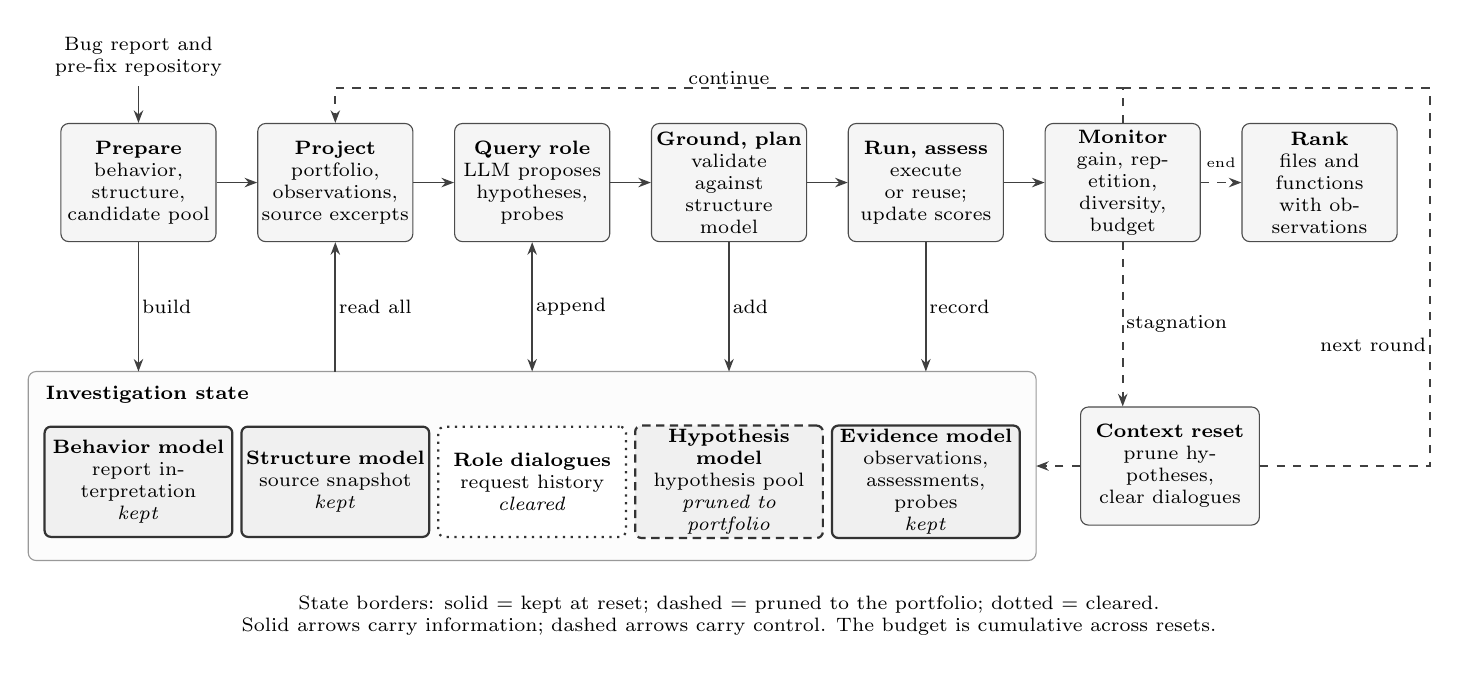
\begin{tikzpicture}[x=1mm,y=1mm,font=\scriptsize,
  stage/.style={draw=black!70,rounded corners=1mm,fill=black!4,align=center,text width=19mm,minimum height=15mm,inner sep=1pt},
  arrow/.style={-{Stealth[length=1.6mm]},semithick,draw=black!75},
  ctrl/.style={arrow,dashed},
  lab/.style={font=\scriptsize,fill=white,inner sep=1pt},
  kept/.style={draw=black!80,thick,fill=black!6,rounded corners=.8mm,align=center,text width=23mm,minimum height=14mm,inner sep=1.2pt},
  pruned/.style={kept,densely dashed},
  cleared/.style={kept,dotted,fill=white}]
% One round of the investigation.
\node[stage] (prep) at (0,0) {\textbf{Prepare}\\behavior, structure,\\candidate pool};
\node[stage] (proj) at (25,0) {\textbf{Project}\\portfolio, observations,\\source excerpts};
\node[stage] (ask) at (50,0) {\textbf{Query role}\\LLM proposes\\hypotheses, probes};
\node[stage] (ground) at (75,0) {\textbf{Ground, plan}\\validate against\\structure model};
\node[stage] (assess) at (100,0) {\textbf{Run, assess}\\execute or reuse;\\update scores};
\node[stage] (mon) at (125,0) {\textbf{Monitor}\\gain, repetition,\\diversity, budget};
\node[stage] (out) at (150,0) {\textbf{Rank}\\files and functions\\with observations};
\node[align=center] (in) at (0,16) {Bug report and\\pre-fix repository};
\draw[arrow] (in)--(prep);
\foreach \a/\b in {prep/proj,proj/ask,ask/ground,ground/assess,assess/mon} \draw[arrow] (\a)--(\b);
\draw[ctrl] (mon)--node[lab,font=\tiny,above=1.5mm]{end}(out);
\draw[ctrl] (mon.north)--(125,12)--node[lab,above]{continue}(25,12)--(proj.north);
% Investigation state and lifetimes at reset.
\draw[draw=black!40,fill=black!1,rounded corners=1mm] (-14,-48) rectangle (114,-24);
\node[anchor=north west,font=\scriptsize\bfseries] at (-13,-24.6) {Investigation state};
\node[kept] (sbeh) at (0,-38) {\textbf{Behavior model}\\report interpretation\\\emph{kept}};
\node[kept] (sstr) at (25,-38) {\textbf{Structure model}\\source snapshot\\\emph{kept}};
\node[cleared] (sdia) at (50,-38) {\textbf{Role dialogues}\\request history\\\emph{cleared}};
\node[pruned] (shyp) at (75,-38) {\textbf{Hypothesis model}\\hypothesis pool\\\emph{pruned to portfolio}};
\node[kept] (sevi) at (100,-38) {\textbf{Evidence model}\\observations,\\assessments, probes\\\emph{kept}};
\draw[arrow] (prep.south)--node[lab,right]{build}(0,-24);
\draw[arrow] (25,-24)--node[lab,right]{read all}(proj.south);
\draw[arrow,{Stealth[length=1.6mm]}-{Stealth[length=1.6mm]}] (ask.south)--node[lab,right]{append}(50,-24);
\draw[arrow] (ground.south)--node[lab,right]{add}(75,-24);
\draw[arrow] (assess.south)--node[lab,right]{record}(100,-24);
% Reset.
\node[stage,text width=22mm] (reset) at (131,-36) {\textbf{Context reset}\\prune hypotheses,\\clear dialogues};
\draw[ctrl] (mon.south)--node[lab,right]{stagnation}(mon.south|-reset.north);
\draw[ctrl] (reset.west)--(114,-36);
\draw[semithick,draw=black!75,dashed] (reset.east)--(164,-36)--node[lab,left,pos=.32]{next round}(164,12)--(125,12);
\node[align=center] at (75,-55) {State borders: solid = kept at reset; dashed = pruned to the portfolio; dotted = cleared.\\Solid arrows carry information; dashed arrows carry control. The budget is cumulative across resets.};
\end{tikzpicture}}
\caption{Overview of \tool{}. The top row shows one round of the investigation; the bottom panel shows the investigation state and what a context reset does to each part. A reset prunes the hypothesis pool to the portfolio and clears all role dialogues and the progress window; every other part of the state, including budget use, is kept, and the next round projects its request from what remains.}\label{fig:flow}
\end{figure}

Because our argument turns on the difference between a fact and a conjecture, the following terms are used in exactly one sense. A \emph{hypothesis} is a candidate location together with a proposed fault mechanism and at least one \emph{prediction}, a condition that can be checked. A \emph{probe} is a planned check of a prediction, an \emph{observation} is the recorded result of running a probe, and an \emph{assessment} states whether an observation supports, contradicts or is inconclusive for a hypothesis. Probes, observations and assessments together form the \emph{evidence}. An \emph{investigator role} is an LLM instruction persona with its own \emph{dialogue}, the history of its requests and responses. A \emph{context reset} clears all dialogues and prunes the hypotheses to a \emph{portfolio}. Each iteration of the investigation is an \emph{attempt}, and an attempt whose LLM response is accepted is a \emph{round}. The \emph{epistemic status} of a model element records whether it was observed, derived by analysis or conjectured. We write ``LLM'' for the language model and reserve ``model'' for the models of the investigation.

Why use models at all? An LLM dialogue is one undifferentiated artifact. Every fact in it is entangled with the conjecture that prompted it and the reasoning that interpreted it, so shortening it by truncation or summarization can drop facts or blur their status. \tool{} instead keeps facts and conjectures as separate elements of models that conform to a metamodel. As Section~\ref{sec:metamodel} explains, the controller keeps each operation's status separate, preserves all observations across resets, and builds every request from the models. After a reset, the request is rebuilt from the stored information rather than the previous dialogue. Between resets, each role's earlier messages are added to its new request. A reset clears this dialogue history.



\subsection{The Investigation Metamodel}\label{sec:metamodel}
A reset can keep facts and drop conjectures only if the investigation state says which is which. The metamodel therefore partitions the state by the kind of knowledge it holds: what the report claims, what the code contains, what the investigator conjectures and what checks have established. Each part becomes a model with its own element types and lifetime, so that the retention decision of Section~\ref{sec:example} can be stated per model rather than per message. Figure~\ref{fig:metamodel} shows the metamodel.

\begin{figure}[pos=H]
\centering
\resizebox{.98\textwidth}{!}{%
\begin{tikzpicture}[x=1mm,y=1mm,font=\scriptsize,
 cls/.style={draw=black!75,fill=white,rectangle split,rectangle split parts=2,rectangle split part align={center,left},text width=21mm,inner sep=1.2pt},
 assoc/.style={draw=black!70,semithick,-{Stealth[length=1.4mm]}},
 comp/.style={draw=black!70,semithick,{Diamond[length=2mm,width=1.4mm]}-{Stealth[length=1.4mm]}},
 ref/.style={assoc,densely dashed},
 mult/.style={font=\fontsize{6}{7}\selectfont,inner sep=.6pt,fill=white},
 pkg/.style={draw=black!35,fill=black!3,rounded corners=1mm,inner sep=2.2mm},
 pkglab/.style={font=\scriptsize\bfseries,anchor=south west,inner sep=1pt}]
\node[cls] (beh) at (0,0) {\textbf{Behavior}\\\stereo{conjectured}\nodepart{two}report\\trigger\\expected, observed\\invariants [*]\\ambiguities [*]};
\node[cls] (sys) at (40,0) {\textbf{Structure}\nodepart{two}revision\\sources (path $\mapsto$ text)\\diagnostics [*]};
\node[cls] (rel) at (40,-27) {\textbf{Relation}\\\stereo{derived}\nodepart{two}kind\\source, target\\resolution};
\node[cls] (loc) at (60,-54) {\textbf{SourceLocation}\nodepart{two}path, line range\\revision, digest\\symbol};
\node[cls] (hyp) at (88,0) {\textbf{Hypothesis}\\\stereo{conjectured}\nodepart{two}mechanism\\assumptions [*]\\causal edges [*]\\score};
\node[cls] (pred) at (88,-27) {\textbf{Prediction}\nodepart{two}description\\predicate\\expected value\\assumptions [*]};
\node[cls] (assess) at (116,-27) {\textbf{Assessment}\nodepart{two}verdict\\scope};
\node[cls] (probe) at (146,0) {\textbf{Probe}\nodepart{two}kind, parameters\\prediction\\cost, reliability};
\node[cls] (obs) at (146,-27) {\textbf{Observation}\\\stereo{observed}\nodepart{two}result\\procedure\\artifact digest};
\draw[comp] (sys.south)--node[mult,right]{relations *}(rel.north);
\draw[comp] (sys.west)--++(-5,0)|-node[mult,above,pos=.75]{symbols *}([yshift=-2mm]loc.west);
\draw[assoc] (rel.south)|-node[mult,above,pos=.75]{location}([yshift=2mm]loc.west);
\draw[comp] (hyp.south)--node[mult,right]{predictions 1..*}(pred.north);
\draw[assoc] (hyp.west)--++(-7,0) coordinate (h1)--(h1|-loc.north) node[mult,pos=.22,left]{locations 1..*};
\draw[assoc] ([yshift=2mm]probe.west)--node[mult,above]{hypothesis}([yshift=2mm]hyp.east);
\draw[assoc] (assess.north)|-node[mult,above,pos=.75]{hypothesis}([yshift=-3mm]hyp.east);
\draw[assoc] (assess.east)--node[mult,above]{obs.}(obs.west);
\draw[assoc] (obs.north)--node[mult,right]{probe}(probe.south);
\draw[assoc] (obs.south)--(146,-66)--node[mult,above]{location}(60,-66)--(loc.south);
\draw[ref] (hyp.north)--(88,19)--node[mult,above]{support, contradictions *}(163,19)--(163,-27)--(obs.east);
\begin{scope}[on background layer]
\node[pkg,fit=(beh)] (pB) {};
\node[pkg,fit=(sys)(rel)(loc)] (pS) {};
\node[pkg,fit=(hyp)(pred)] (pH) {};
\node[pkg,fit=(probe)(assess)(obs)] (pE) {};
\end{scope}
\node[pkglab] at (pB.north west) {Behavior model};
\node[pkglab] at (pS.north west) {Structure model};
\node[pkglab] at (pH.north west) {Hypothesis model};
\node[pkglab] at (pE.north west) {Evidence model};
\end{tikzpicture}}
\caption{The investigation metamodel. A stereotype abbreviates a status attribute set at creation and never changed: LLM-derived elements are conjectured, extracted relations are derived, and probe results are observed. Diamonds denote containment. The associations from Probe, Assessment and Observation to hypotheses, observations and probes, and the dashed support and contradiction links, are references by identifier; the others hold the referenced objects. Role dialogues are not part of the metamodel.}\label{fig:metamodel}
\end{figure}

\emph{Behavior model.} This model holds the report together with the latest LLM interpretation of it: a trigger, the expected and the observed behavior, candidate invariants and ambiguities. Each accepted LLM response replaces the trigger and the expected and observed behavior. In the evaluated version, ambiguities were appended rather than replaced, a defect whose consequences we discuss in Sections~\ref{sec:runtime} and~\ref{sec:threats}. When the expected or observed behavior is missing, the model records the gap as an ambiguity. The fields are conjectures, but they give every role the same statement of the discrepancy to explain.

\emph{Structure model.} This model is a snapshot of the production Python files at the fixed revision. It stores each file's text, class and function symbols with their line ranges, and relations: imports, calls, reads, writes and intraprocedural data flow. Every symbol and relation location carries the file's content digest. A call to a top-level definition or an explicitly imported name is marked as syntactically resolved; other calls are marked unresolved. The structure model is built once per run, and it serves to expand the candidate pool and to ground the locations that investigators propose.

\emph{Hypothesis model.} This model is the pool of live hypotheses. A hypothesis names one file and one or more locations in it, a mechanism in natural language, one or more predictions, optional causal edges (conjectured links along which the fault propagates between locations), links to supporting and contradicting observations, and a score. A prediction consists of a description, a predicate, an expected value and assumptions. A hypothesis is identified by its file, its case-folded mechanism and the kind of probe that accompanies it; when an investigator proposes the same hypothesis again, new locations and predictions are merged into the existing element.

\emph{Evidence model.} This model holds probes, observations and assessments. A probe names its hypothesis, the prediction it checks, a probe kind and parameters. An observation records the probe's result, the procedure that produced it, the source location with revision and file digest, and the digest of a stored artifact. An assessment links an observation to a hypothesis with a verdict and the scope of what was observed: source presence, static structure or execution. Observations are identified by their content. Controller operations do not modify or delete them, and probes that perform the same check reuse one observation. Probe objects themselves are transient; what persists is each observation with the identifier of its probe, a cache of executed checks and the set of probes already handled.

Table~\ref{tab:models} summarizes the four models and what a reset does to each. The dialogues of the investigator roles appear as a fifth row because they are the part of the state that a reset clears, but they are deliberately kept outside the metamodel.

\begin{table*}[width=\FullWidth,pos=!htbp]
\caption{The four models of an investigation and their lifetime at a context reset.}\label{tab:models}
\centering\small\setlength{\tabcolsep}{3pt}
\renewcommand{\arraystretch}{1.12}
\begin{tabular}{@{}>{\raggedright\arraybackslash}p{.13\textwidth}>{\raggedright\arraybackslash}p{.29\textwidth}>{\raggedright\arraybackslash}p{.27\textwidth}>{\raggedright\arraybackslash}p{.11\textwidth}>{\raggedright\arraybackslash}p{.13\textwidth}@{}}\toprule
Model & Content & Used for & Status & At a reset\\\midrule
Behavior & Report; trigger; expected and observed behavior; invariants; ambiguities & Shared statement of the discrepancy in every request & Conjectured (except the report) & Kept (latest interpretation)\\
Structure & File texts; symbols; import, call and data-flow relations; digests & Candidate expansion; grounding of proposed locations & Derived & Kept (built once)\\
Hypothesis & Hypotheses with locations, mechanism, predictions, links to observations, score & Portfolio shown in each request; final ranking & Conjectured & Pruned to the portfolio\\
Evidence & Observations with provenance; assessments; probe cache and handled probes & Assessment, progress monitoring, projection & Observed & Kept, append-only (probes are transient)\\
\midrule
Role dialogues & Requests and responses of each role (not a model) & Conversational continuity within a role & -- & Cleared\\
\bottomrule\end{tabular}
\end{table*}

Separating the models is not enough on its own. An operation that turned a conjecture into an observation, lost the revision of a checked file or dropped an observation at a reset would silently undo the separation. We therefore state four invariants that every operation of Section~\ref{sec:operations} must maintain. I1 keeps facts and conjectures apart, I2 ties every fact to the inspected source, I3 keeps the links between them consistent, and I4 is the preservation obligation of a reset.
\begin{description}
\item[I1] \emph{Epistemic separation.} The status of an element is set by the operation that creates it, and no operation changes it. Observations are created only by running probes; relations only by structure extraction; behavior fields only from the report and LLM proposals; hypotheses and causal edges only from LLM proposals. Grounding marks every proposed causal edge as conjectured, whatever certainty the LLM claims, and assessment changes a hypothesis's score and links but not its status.
\item[I2] \emph{Source traceability.} Every hypothesis location and every observation carries the revision and the content digest of its file. The evidence model rejects an observation from another revision, one without procedure and digest provenance, or one whose artifact fails an integrity check, and the controller rejects an observation whose file digest differs from the structure model's.
\item[I3] \emph{Referential integrity.} Every support or contradiction link of a live hypothesis resolves to a recorded observation. The links are checked against the evidence model after each assessment, and against the observations the role may access whenever the hypothesis is projected into a request.
\item[I4] \emph{Observation preservation.} Controller operations neither modify nor delete observations. Insertion checks reject changed records under an existing identifier except for the originating probe identifier; nested result dictionaries are not deeply immutable (Appendix~\ref{app:realization}). A context reset leaves the set of observation identifiers unchanged, which the controller asserts at runtime, and it neither refunds nor resets the budget.
\end{description}
The metamodel is implemented as Python dataclasses rather than in a modeling framework such as EMF. I1 holds by construction, because no operation assigns a status after creation and grounding overwrites the status of every proposed causal edge; I2--I4 are enforced by explicit checks in the evidence model, the operations and the controller (Appendix~\ref{app:code-correspondence}). These checks guard the invariants at runtime, but they are not a proof. The I4 assertion, for example, compares the observation identifiers before and after a reset. Because the reset code never touches the evidence model, the assertion guards against future regressions rather than proving a property, and it is removed when Python runs with optimizations (\code{-O}). Status is fixed per element type and keeps facts and conjectures apart in requests and assessments; it does not drive control decisions. Assessments of pruned hypotheses remain in the evidence model as history but are no longer shown.

\subsection{Model Operations}\label{sec:operations}
The models change only through a fixed set of operations, and this is what makes the invariants checkable. Each operation has a declared input and output model, so it is clear which operation may create an observation, which may only create a conjecture and which may only select. In MDE terms, extraction operations are text-to-model and code-to-model transformations, grounding and planning are model-to-model transformations, and projection is a model-to-view transformation whose result is the LLM request. Table~\ref{tab:operations} lists the operations. In its signatures, $r$ is the report, $R$ and $v$ the repository and revision, $z$ an accepted LLM response with proposals $z_j$, and $\psi_j$ the probe parameters of proposal $j$; $s$, $b$, $h$, $p$, $e$ and $a$ denote a structure model, behavior model, hypothesis, probe, observation and assessment, and $H$, $S$, $E$, $B$, $A$ and $\Omega$ the hypothesis pool, portfolio, evidence model, budget, role dialogues and progress window.

\begin{table*}[width=\FullWidth,pos=!htbp]
\caption{Model operations of \tool{}.}\label{tab:operations}
\centering\small\setlength{\tabcolsep}{3pt}
\renewcommand{\arraystretch}{1.12}
\begin{tabular}{@{}>{\raggedright\arraybackslash}p{.13\textwidth}>{\raggedright\arraybackslash}p{.14\textwidth}>{\raggedright\arraybackslash}p{.2\textwidth}>{\raggedright\arraybackslash}p{.47\textwidth}@{}}\toprule
Operation & Kind & Signature & Responsibility\\\midrule
Extract behavior & Text to model & $(r,z)\mapsto b$ & Copy the LLM's interpretation of the report; record missing expected or observed behavior as an ambiguity\\
Extract structure & Code to model & $(R,v)\mapsto s$ & Parse production files; record symbols, relations and digests; keep syntax errors as diagnostics\\
Expand & Model query & $(s,\textit{seeds})\mapsto\textit{files}$ & Two-hop, bidirectional neighborhood of the seed files over relations not marked unresolved\\
Ground & Proposal to model & $(z_j,s)\mapsto h$ & Validate file, line, mechanism and prediction; attach revision, digest and enclosing symbol; mark causal edges conjectured\\
Plan & Model to model & $(h,\psi_j)\mapsto p$ & Build a typed probe from the investigator-specified kind and parameters\\
Assess & In-place update & $(h,p,e)\mapsto(h',a)$ & Compare the observed value with the prediction; link the observation; change the score\\
Project & Model to view & $(b,S,E,B)\mapsto x$ & Build the request view of hypotheses, observations, unresolved predictions and budget\\
Reset & Selection & $(H,A,\Omega)\mapsto(S,\varnothing,\varnothing)$ & Prune the pool to the portfolio; clear dialogues and the progress window; preserve everything else\\
\bottomrule\end{tabular}
\end{table*}

\emph{Extraction.} \textsc{ExtractStructure} parses every production Python file with Python's \code{ast} module, skipping test directories and test files. Files that fail to parse remain retrievable but contribute only a diagnostic.

\emph{Candidate preparation.} \tool{} first ranks all files against the report with BM25, a term-based retrieval function~\citep{bm25_2009}. The five highest-ranked files seed \textsc{Expand}, which collects the files reachable within two hops in either direction over relations not marked unresolved. Data-flow relations stay within a file, so in practice the neighborhood follows imports and calls. The candidate pool consists of the seeds, then the neighborhood files in BM25 order, then the remaining files in BM25 order, truncated to 20 files, and it is fixed for the run. In a larger version of the running example, the import and call from \code{handle} to \code{normalize} would bring \code{config.py} into the pool even if BM25 ranked it below the seeds. Only pool files are ever shown to the investigator, so the pool bounds which files can receive hypotheses.

\emph{Grounding and planning.} \tool{} considers the first four proposals of a response, each with a file, a mechanism, a prediction and a probe. \textsc{Ground} accepts a proposal only if its file was shown in the request, the proposed line exists in that file, the probe targets the same file, and the mechanism and prediction are nonempty. It then builds a source location with the revision, the file digest and the narrowest enclosing symbol, and it adds the hypothesis to the pool or merges it with an existing one. \textsc{Plan} turns the investigator's probe specification into a typed probe of one of five kinds: a source quote, an AST query, a test, a trace or a counterfactual comparison of two procedures. The investigator, not \tool{}, chooses the check, and \tool{} never synthesizes tests from a mechanism. The probe kind is checked when planning and the kind-specific parameters when the probe runs; a hypothesis whose probe proves malformed stays in the pool with score zero.

\emph{Running probes.} A source-quote probe checks whether a quoted text occurs on a given line. An AST query checks whether the file contains a node of an allowed type, such as a \code{return} statement, whose source text contains a given string; the whole file is searched. Tests, traces and counterfactuals run only as procedures registered by the experimenter in an isolated container, and an unregistered request is recorded as a blocked observation. Two mechanisms avoid repeated work. First, a check, identified by probe kind, file and parameters, executes at most once per run: if another hypothesis already ran it, the recorded observation is reused and assessed for the new hypothesis, but it does not count as new. Second, if the same hypothesis already ran a probe with the same kind and parameters, the probe is skipped and nothing is assessed.

\emph{Assessment.} \textsc{Assess} reads the observed value that the prediction's predicate refers to---for an AST query, whether any node matched---and compares it with the expected value. Equal values support the prediction, unequal values contradict it, and a missing value, a blocked or timed-out procedure, or a predicate that does not fit the probe kind is inconclusive. A hypothesis's score is the signed sum of the weights of its assessments,
\begin{equation}\label{eq:score}
\mathrm{score}(h)=\sum_{e\in\mathrm{Sup}(h)} w(h,e)-\sum_{e\in\mathrm{Con}(h)} w(h,e),
\end{equation}
where $\mathrm{Sup}(h)$ and $\mathrm{Con}(h)$ are the supporting and contradicting observations, and $w(h,e)$ is 0.25 when $e$ was assessed for $h$ against a source-presence prediction, 1 for a structural prediction checked by an AST query, and 2 for a prediction checked by execution. The weights encode the relative strength of the three kinds of check; they are chosen ordering priorities, not probabilities. An additive score is the simplest aggregate in which contradictions offset support. It treats observations as independent, a simplification we revisit in Section~\ref{sec:threats}. Each hypothesis--observation pair contributes to the score at most once.

\emph{Projection.} \textsc{Project} builds the request view from the behavior model, the current portfolio, the observations accessible to the role and the remaining token budget. Each hypothesis appears with its locations, its mechanism labeled as unverified, its predictions, its conjectured causal edges, and the identifiers of its supporting observations (split into static and execution-based) and of its contradicting observations. Predictions of hypotheses without execution support are listed as unresolved. The view lists hypotheses in portfolio order and shows no scores. The controller then adds numbered excerpts of up to four pool files, their BM25 ranks and up to twelve structural relations from those files. The first request shows the four leading candidates; later requests show the BM25 leader and the file of the first portfolio hypothesis and rotate through the rest of the pool. The role's dialogue, if any, precedes the new request. Because projection runs before every request, a reset needs no separate reconstruction step.

\subsection{The Investigation Loop}\label{sec:procedure}
The operations say how the models change, but not in which order or when to stop. A localization investigation must interleave asking the LLM, checking its proposals and deciding whether to continue, while keeping every LLM call inside a cumulative budget and giving the reset policy a defined point at which to act. Algorithm~\ref{alg:controller} gives the loop that ties the operations together, and we describe it in line order. Lines~\ref{alg:prep-start}--\ref{alg:prep-end} prepare the structure model, the behavior model, the BM25 ranking $L$ and the candidate pool $C$, and they initialize the hypothesis pool $H$, the evidence model $E$ (including the probe cache and the set of handled probes), the role dialogues $A$ and the progress window $\Omega$.

\algtext*{EndIf}\algtext*{EndFor}
\begin{algorithm}[!htbp]
\caption{The \tool{} investigation loop}\label{alg:controller}
\begin{algorithmic}[1]\small
\Require report $r$; repository $R$ at revision $v$; attempt limit $N$; budget $B$ (tokens, probes, time); portfolio bound $m$
\Ensure ranked files and functions; evidence model $E$
\State $s\gets\textsc{ExtractStructure}(R,v)$\label{alg:prep-start}
\State $b\gets\textsc{ExtractBehavior}(r,\varnothing)$\label{alg:behavior}
\State $L\gets\textsc{BM25}(r,s)$;\; $C\gets\textsc{Pool}(L,\textsc{Expand}(s,L_{1..5}))$\label{alg:pool}
\State $H,E,A,\Omega\gets\varnothing$;\; $n\gets0$\label{alg:prep-end}
\For{$i\gets1$ \textbf{to} $N$}
  \If{$\textsc{Exhausted}(B)$}\label{alg:admit} \State \textbf{break} \EndIf
  \State $\rho\gets\textsc{Role}(i)$;\; $S\gets\textsc{Portfolio}(H,m)$\label{alg:select}
  \State $F\gets\textsc{Files}(C,L,S,i)$
  \State $x\gets\textsc{Project}(b,S,E,B)\oplus\textsc{Excerpts}(F)$\label{alg:project}
  \State $z\gets\textsc{Ask}(\rho,A_\rho,x)$ \Comment{charges tokens to $B$}\label{alg:ask}
  \If{$z=\bot$}\label{alg:reject} \State \textbf{continue} \Comment{rejected response} \EndIf
  \State $A_\rho\gets A_\rho\cdot(x,z)$;\; $b\gets\textsc{ExtractBehavior}(r,z)$\label{alg:accept}
  \State $n\gets n+1$ \Comment{accepted rounds}
  \State $(H,P)\gets\textsc{GroundAndPlan}(z,s,H,F)$\label{alg:ground}
  \State $(H,E)\gets\textsc{RunAndAssess}(P,H,E,B)$\label{alg:run}
  \State $\Omega\gets\textsc{Record}(\Omega,H,E,P,B)$\label{alg:record}
  \State $H^{-}\gets H$ \Comment{pool before any reset}
  \If{$\textsc{Stagnated}(\Omega,n,B)$}\label{alg:stagnated}
    \State $H\gets\textsc{Portfolio}(H,m)$;\; $A\gets\varnothing$;\; $\Omega\gets\varnothing$ \Comment{reset}\label{alg:reset}
  \EndIf
  \If{$\textsc{ExecutionStop}(H^{-},E)$}\label{alg:stop} \State \textbf{break} \EndIf
\EndFor
\State \Return $\textsc{Rank}(L,H)$, $E$\label{alg:rank}
\end{algorithmic}
\end{algorithm}

Each iteration of the loop is one attempt. The loop ends early when the token, probe or time budget is exhausted (line~\ref{alg:admit}); the LLM backend can also end the run when a request no longer fits the remaining budget or the context window. Roles follow a fixed schedule---behavioral, skeptical, structural, dynamic---and share the models but not their dialogues. The behavioral role separates report claims from observations, the skeptical role tries to falsify the leading hypothesis and keep a distinct alternative, the structural role traces dependencies, and the dynamic role proposes registered tests or traces and falls back to static queries.

Lines~\ref{alg:select}--\ref{alg:project} select the portfolio $S$ and the files $F$ to show and project the request; $\oplus$ appends the source excerpts to the projected view. A response that is not a well-formed object with a list of hypotheses is rejected (line~\ref{alg:reject}): it consumes the attempt and its tokens but changes no state. An accepted response is appended to the role's dialogue $A_\rho$, refreshes the behavior model and yields the planned probes $P$ (lines~\ref{alg:accept}--\ref{alg:ground}); invalid proposals are skipped individually. Line~\ref{alg:run} runs the probes not yet handled, in the order described in Section~\ref{sec:portfolio}, and assesses their results. Line~\ref{alg:record} records the round's progress, and lines~\ref{alg:stagnated}--\ref{alg:reset} reset the context when the investigation stagnates (Section~\ref{sec:reset}). If execution procedures are registered, the run can also stop once the leading hypothesis has support from two distinct procedures, stated assumptions and no contradiction (line~\ref{alg:stop}). This check inspects the pool $H^{-}$ as it was before any reset in the same round, and in a source-only configuration it never holds. Finally, line~\ref{alg:rank} produces the ranking (Section~\ref{sec:output}).

\subsection{The Hypothesis Portfolio}\label{sec:portfolio}
The portfolio decides which hypotheses the investigator sees. Showing every hypothesis would let near-duplicates crowd out alternatives, and showing only the leader would reproduce the restart-from-best problem of the motivating example. \tool{} therefore selects hypotheses by score and diversity, in the spirit of maximal marginal relevance in retrieval~\citep{mmr1998}. Diversity rests on a dissimilarity between hypotheses,
\begin{equation}\label{eq:distance}
\begin{aligned}
D(h,h')={}&0.6\left(1-\frac{|\tau(h)\cap\tau(h')|}{\max(1,|\tau(h)\cup\tau(h')|)}\right)\\
&+0.4\,\mathbf{1}[\pi(h)\neq\pi(h')],
\end{aligned}
\end{equation}
where $\tau(h)$ is the set of lowercase alphabetic words of at least three letters in the mechanism of $h$ and $\pi(h)$ is its file. $D$ ranges over $[0,1]$ and combines how differently two mechanisms are worded with whether they concern different files. The portfolio $S=\textsc{Portfolio}(H,m)$ is built greedily. Starting from $S_0=\varnothing$,
\begin{equation}\label{eq:portfolio}
\begin{aligned}
S_{j+1}&=S_j\cup\{h_{j+1}\},\\
h_{j+1}&=\operatorname*{arg\,max}_{h\in H\setminus S_j}\Bigl[\mathrm{score}(h)+\min_{h'\in S_j}D(h,h')\Bigr],
\end{aligned}
\end{equation}
with the minimum over an empty set taken as 1, until $|S|=m$ or $H$ is exhausted; ties go to the higher score and then the smaller identifier. The first choice is thus the highest-scored hypothesis, and each later choice trades score against difference from those already chosen. Because $D$ is at most 1, diversity reorders only hypotheses whose scores differ by less than one, the weight of a single AST check, and among those it prefers hypotheses that differ in wording or file from the ones already chosen. The default bound is $m=3$.

Within a round, \tool{} runs every unhandled probe. It orders them by a utility that prefers inexpensive static probes, probes whose prediction contrasts with those of other hypotheses, and probes of hypotheses that differ from the rest of the pool (Appendix~\ref{app:ordering}). The order matters only when the probe or time ceiling is reached in the middle of a round.

\subsection{Stagnation Detection and Context Reset}\label{sec:reset}
The reset policy is meant to act when observable progress stalls, and its timing involves a trade-off. Resetting too early discards each role's line of reasoning while it is still producing new checks. Resetting too late lets the investigation keep re-proposing the same checks and converging on near-identical explanations, as in rounds 2--4 of the running example. The reset rule therefore watches for the observable signs of the second situation: rounds that add no new observation while the investigation either repeats executed checks or loses diversity among its hypotheses.

After each accepted round $t$, the monitor records four quantities: the number $g_t$ of new observations that are not blocked; the fraction $u_t$ of the round's probes whose check (kind, file and parameters) had already been executed (zero if the round has no grounded probe); the pool diversity $d_t$, the mean of $D$ over all pairs of live hypotheses (zero for fewer than two); and the tokens $\kappa_t$ the round consumed. The window $\Omega$ holds the samples of the last $W$ accepted rounds since the start or the most recent reset, and $n$ counts accepted rounds since the start. The investigation has stagnated when
\begin{equation}\label{eq:reset}
\begin{aligned}
&n\ge n_0\;\wedge\;|\Omega|=W
&&\text{(ready)}\\
\wedge\;&\bar g\le\theta_g\;\wedge\;(\bar u\ge\theta_u\vee\bar d<\theta_d)
&&\text{(stalled)}\\
\wedge\;&B_{\mathrm{rem}}>\max\bigl(\kappa_0,\lfloor\kappa_t/2\rfloor\bigr)+\kappa_0
&&\text{(affordable)},
\end{aligned}
\end{equation}
where $\bar g$, $\bar u$ and $\bar d$ are window means and $B_{\mathrm{rem}}$ is the remaining token budget. The defaults are $W=3$, $n_0=4$, $\theta_g=0$, $\theta_u=\theta_d=0.5$ and a reserve of $\kappa_0=256$ tokens. With $\theta_g=0$, the gain condition requires that the last three rounds produced no new observation at all. Appendix~\ref{app:reset} lists two further conditions: an optional consumed-fraction gate, which is vacuous under the defaults, and a requirement that the window's rounds consumed at least $\kappa_0$ tokens, which realistic LLM rounds satisfy.

Each condition encodes a judgment. Judging gain over a window rather than a single round avoids resetting after one unproductive response. Requiring repetition or low diversity is intended to distinguish an investigation that circles, re-proposing executed checks or converging on similar hypotheses, from one that explores without immediate success. The budget condition requires the remaining tokens to exceed a reserve plus half the tokens of the latest round, a heuristic estimate of the cost of a fresh request that does not guarantee that a full further round fits. The thresholds are design parameters rather than calibrated values, and Section~\ref{sec:rq2} reports how often the default policy acted in practice.

A reset (line~\ref{alg:reset} of Algorithm~\ref{alg:controller}) prunes the hypothesis pool to the portfolio, clears every role dialogue and the progress window, and changes nothing else. The behavior and structure models, all observations and assessments, the probe cache, the set of handled probes, the accepted-round count $n$ and the cumulative budget remain. Because the window is cleared while $n$ is kept, two resets are at least $W$ accepted rounds apart.

The effects of a reset unfold at two times. Immediately, the next request no longer carries any dialogue. Because each dialogue turn stores the full request that produced it, a long dialogue holds several stale copies of earlier state, and the reset removes them. The dialogue is, however, also the only place where excerpts of files no longer displayed persist, and it preserves each role's line of reasoning; a reset trades this continuity for a request free of stale state, and the fixed-reset and continuous-context workflows of our study bracket that trade-off. The visible portfolio does not change at the moment of the reset, since the portfolio of a pruned pool is the pool itself. Pruning acts later: pruned hypotheses can no longer re-enter the portfolio, count toward diversity or influence the final ranking. A reset therefore forgets interpretations as well as dialogue. We made this choice deliberately. At a stagnation point, the hypotheses outside the portfolio are those that score and diversity already rank below $m$ others, and pruning them keeps the diversity signal and the final ranking focused on the explanations the investigation is still pursuing. If a pruned hypothesis is proposed again, it returns with a zero score and without its former links, and its earlier probe is not rerun because it has already been handled. Observations remain recorded (I4) and available to the next projection, although I4 does not guarantee that every record fits the backend's context window.

\subsection{Producing the Ranking}\label{sec:output}
When the loop ends, \textsc{Rank} orders files by the highest score of a live hypothesis in each file. A file without a live hypothesis receives score $-1$, and BM25 order breaks ties, so lexical retrieval serves as the fallback. This rule has a consequence that is central to interpreting our results. A file whose hypothesis was proposed but not yet checked (score 0), or contradicted only by a source-presence check ($-0.25$), still ranks above every uninvestigated file, so the LLM's proposals can reorder the BM25 list without supporting evidence. Conversely, an investigation that ends with no live hypothesis returns exactly the BM25 order. The function ranking lists the enclosing symbols of live hypotheses' locations in decreasing order of score and has no lexical fallback.

The output also contains the observations and assessments, so hypothesis-backed locations can be traced to the checks that support them; retrieval-only entries and unchecked hypotheses have no such support. \tool{} reports no confidence value. Its abstention flag is cleared by any supporting execution-based assessment in the run, including one for a non-leading or pruned hypothesis, so the flag does not certify the leading location (Appendix~\ref{app:termination}). It remains set for source-only runs.

\subsection{The Running Example, End to End}\label{sec:trace}
Table~\ref{tab:trace} follows the running example through Algorithm~\ref{alg:controller}, and Table~\ref{tab:synthetic} in Appendix~\ref{app:reset} spells out the reset arithmetic. Scripts in the replication package check both against the implementation. The last row shows what the portfolio adds: with a leader-only bound, the refuted bypass idea could return without the link that records its refutation.

\begin{table}[pos=!htbp]
\caption{The running example traced through \tool{}, with hypotheses $h_b$ (bypass) and $h_d$ (defaulting).}\label{tab:trace}
\centering\footnotesize\setlength{\tabcolsep}{3pt}
\renewcommand{\arraystretch}{1.1}
\begin{tabular}{@{}>{\raggedright\arraybackslash}p{.15\columnwidth}>{\raggedright\arraybackslash}p{.80\columnwidth}@{}}\toprule
Step & What happens\\\midrule
Prepare & The structure model records \code{handle} and \code{normalize}, an import of \code{config.py}, and a call from \code{handle} to \code{normalize}; the call to \code{render} is unresolved. Both files are BM25 seeds, and \code{config.py} is also reachable from \code{handler.py} through the import and call.\\
Round 1 & The behavioral role sees the report and both files. It records the trigger and the expected and observed behavior, and proposes $h_b$ and $h_d$ with AST probes whose predictions use the predicate \code{ast_matches} with expected value true.\\
Ground & $h_b$ is placed at \code{handler.py:4} in \code{handle}, $h_d$ at \code{config.py:2} in \code{normalize}, each with revision and file digest.\\
Assess & No \code{return} in \code{handler.py} contains \code{options}: $h_b$ is contradicted, score $-1$. The \code{return} in \code{config.py} contains \code{or True}: $h_d$ is supported, score $+1$.\\
Rounds 2--4 & The skeptical, structural and dynamic roles re-propose the executed checks. Each round adds no observation ($g_t=0$) and repeats every probe ($u_t=1$).\\
Reset & After round 4, $n=4$, the window is full, $\bar g=0$, $\bar u=1$, and the budget suffices. The pool is pruned to the portfolio $(h_d,h_b)$; dialogues and window are cleared; observations, scores and budget are unchanged.\\
Round 5 & The request carries the behavior model, $h_d$ and $h_b$, both observations and the remaining budget, but no earlier dialogue.\\
Rank & \code{config.py} (score $1$) ranks first; \code{handler.py} ties at $-1$ with uninvestigated files and is placed by BM25. Functions: \code{normalize}, then \code{handle}.\\
Leader only & With $m=1$, every request shows only $h_d$, and the reset discards $h_b$. If a later round proposes the bypass idea again, $h_b$ returns with score 0 and no links, and its probe is skipped as already handled; the refuting observation stays in the request but is no longer linked to it.\\
\bottomrule\end{tabular}
\end{table}

\subsection{Scope and Assumptions}\label{sec:scope}
Several boundaries apply throughout. \tool{} targets Python, and its structure model is approximate. Calls are resolved syntactically, dynamic dispatch stays unresolved, and the two-hop neighborhood is a heuristic rather than a semantic slice; because import targets outside the repository are traversed, widely imported standard-library modules act as hubs at the second hop and can make the neighborhood broad. The stagnation monitor counts an observation as new by its identity, which includes the probe parameters, so a slightly reworded quote counts as new evidence. Scores and dissimilarities are heuristics, not probabilities. The fixed candidate pool bounds recall, and retaining every observation does not bound the size of later requests. Finally, a reset preserves observations but not the interpretations attached to pruned hypotheses. Appendix~\ref{app:implementation} documents the remaining operational details.

\section{Study Design}\label{sec:study}
The study asks how the retention policy of a localization agent affects its rankings, its use of resources and the investigation it actually carries out. It does not ask whether \tool{} outperforms other localizers. This goal, together with the way \tool{} produces its output, shaped three decisions that run through the design. We explain them first and then describe the workflows, subjects, runtime and measures.

\subsection{Design Rationale}\label{sec:rationale}
\emph{Comparing policies within one implementation.} A comparison of \tool{} against external agents would confound the context policy with differences in tools, prompts, navigation and candidate retrieval, any of which can affect localization accuracy as much as the policy itself. Because \tool{} expresses every workflow as a configuration of the same controller rather than as separate code (Appendix~\ref{app:code-correspondence}), the workflows share grounding, probe execution, scoring, excerpt construction, role instructions and ranking, and they differ only in what requests show and what resets do. The comparison is therefore a controlled contrast of context policies. The price is that it says nothing about competitiveness with complete localization systems, a question we leave to future work.

\emph{Pairing on issues.} Localization difficulty can be expected to vary far more between issues than between context policies, so we run every workflow on every issue with each LLM and compare workflows issue by issue. Pairing removes issue difficulty from each contrast and lets us report exactly which issues a workflow gains or loses relative to another, instead of only comparing aggregate rates.

\emph{Measuring the investigation, not only the ranking.} As Section~\ref{sec:output} explains, an investigation that ends without a live hypothesis returns the BM25 order. A workflow whose investigations fail could thus score exactly like retrieval, and two workflows with equal accuracy could differ completely in how much investigative work stands behind their rankings. We therefore add two retrieval controls that show what the LLM adds to the ranking, and process measures that show whether the investigation produced usable output at all. For the same reason, an adaptive policy can only matter where it acts, so a null result for adaptive resets is uninterpretable without knowing how often resets occurred.

These decisions translate directly into the research questions of Section~\ref{sec:intro}. RQ1 compares the rankings a developer would receive. RQ2 measures reset exposure, which is the precondition for any effect of a reset policy, and uses the fixed schedule to separate the question of \emph{whether} to reset from \emph{when}. RQ3 asks whether a policy trades accuracy for cost under a common ceiling, since policies change request length and output volume. RQ4 examines final hypothesis pools and response diagnostics, which the retrieval fallback makes necessary.

\subsection{Context Workflows}\label{sec:variants}
Table~\ref{tab:variants} defines the evaluated configurations. They were chosen to cover the retention space between never forgetting and forgetting everything but the facts. \emph{Continuous context} is the no-forgetting baseline: it keeps every dialogue and every live hypothesis and never resets. \emph{Full adaptive}, the \tool{} design of Section~\ref{sec:approach}, projects the model state together with each role's dialogue and resets and prunes on stagnation. \emph{Fixed reset} applies the same reset operation after every third attempt, provided that attempt was accepted, without consulting the monitor; comparing it with full adaptive separates the effect of resetting from the effect of the monitor's timing. The \emph{observation-only view} sits at the opposite end from continuous context: each request is rebuilt from scratch and shows the report and the recorded observations, but none of the investigator's earlier hypotheses or dialogue. It tests whether showing hypotheses to the investigator helps at all. Finally, the BM25 and graph retrieval controls rank files without an LLM, which measures how much of each workflow's accuracy the retrieval fallback already provides.

\begin{table}[pos=!htbp]
\caption{Evaluated configurations. Dialogue and hypothesis-pool retention are part of the treatment.}\label{tab:variants}
\centering\small
\begin{tabular*}{\textwidth}{@{\extracolsep{\fill}}p{.20\textwidth}p{.24\textwidth}p{.48\textwidth}@{}}\toprule
Workflow & Artifact name & Memory and reset policy\\\midrule
Full adaptive & \code{morph} & Project model state plus role dialogue; reset and prune on stagnation\\
Continuous & \code{no_forgetting} & Keep dialogue and all live hypotheses; no resets\\
Fixed reset & \code{fixed_reset} & Same reset and pruning operation every third attempt if that attempt is accepted\\
Observation-only & \code{stateless_summary} & Report and compact observations as memory; no dialogue, resets or pruning\\
BM25 / Graph & \code{bm25}, \code{graph} & File retrieval; no LLM and no function ranking\\\bottomrule
\end{tabular*}
\end{table}

All four LLM workflows share grounding, source and probe validation, evidence processing, scoring, the rules for constructing source excerpts, role instructions and ranking, and within each LLM they use the same checkpoint and resource ceilings. Because evolving hypotheses influence which files are displayed, the source a workflow shows downstream need not be identical across workflows; this is part of the treatment.

The observation-only view needs a closer description, because it differs from the other workflows in more than one respect. It retains the common numbered source excerpts, retrieval ranks, revision and instructions. It omits hypotheses, the interpreted behavior, unresolved predictions, relations, the displayed budget and detailed provenance. Its artifact name is historical and does not refer to an LLM-written summary; observations are listed as recorded. Internally, the workflow still keeps hypotheses, grounds and checks proposals and uses their scores to rank locations, and because it never resets, its unpruned pool can affect the final ranking. The contrast with the other workflows therefore bundles several changes, and it cannot isolate the effect of removing dialogue, removing hypotheses or omitting any individual field. In addition, all workflows store evidence externally, so none of them measures the benefit of preserving observations against deleting them. We return to these limits in Section~\ref{sec:threats}.

\subsection{Subjects}\label{sec:subjects}
We draw subjects from SWE-bench Lite and SWE-bench Verified~\citep{swebench2024,swebenchverified2024}. Both provide real issues from popular Python projects together with the pre-fix repository snapshot and the reference patch, which is what report-based localization requires, and both are widely used to evaluate LLM agents. The two splits contain 300 and 500 issues and share 93, giving 707 unique issues; an issue in both enters our sample once.

We selected 50 issues. A few repositories, Django above all, contribute a large share of the benchmark issues, so a random sample would mostly measure behavior on those projects. We therefore selected issues round-robin across twelve repositories, in deterministic hash order within each repository, after excluding thirteen issues that had been inspected during development. The selected identifiers were fixed before any prediction or label for this selection was opened. Balancing limits the influence of any single project at the price of changing the benchmark's mixture, so the sample is not representative of either split. Its size reflects the cost of a complete paired design: each issue is investigated eight times, and we preferred covering two LLMs on every issue to covering more issues with one. Table~\ref{tab:eval-coverage} gives the repository composition. All 50 issues have file targets and 48 have function targets.

\begin{table}[pos=!htbp]
\caption{Repository composition of the fixed 50-issue sample. Function eligibility is determined separately by nonempty patch-derived targets.}\label{tab:eval-coverage}
\centering\small
\begin{tabular*}{\textwidth}{@{\extracolsep{\fill}}lrr@{}}\toprule
Repository & Issues & Function-eligible\\\midrule
astropy/astropy & 5 & 5\\
django/django & 5 & 5\\
matplotlib/matplotlib & 5 & 5\\
mwaskom/seaborn & 4 & 4\\
pallets/flask & 3 & 3\\
psf/requests & 4 & 4\\
pydata/xarray & 4 & 4\\
pylint-dev/pylint & 4 & 3\\
pytest-dev/pytest & 4 & 4\\
scikit-learn/scikit-learn & 4 & 4\\
sphinx-doc/sphinx & 4 & 4\\
sympy/sympy & 4 & 3\\
\midrule Total & 50 & 48\\
\bottomrule\end{tabular*}
\end{table}

Investigators receive the public report and the pre-fix source. The reference patches are visible only to the evaluator, which derives the changed files and functions as localization targets. These targets are proxies for the fault location rather than adjudicated root causes, as we discuss in Section~\ref{sec:threats}.

\subsection{LLMs, Budget and Evidence}\label{sec:runtime}
\emph{LLMs.} We use two open code LLMs from different model families, Qwen2.5-Coder-7B-Instruct~\citep{qwen25coder2024} and DeepSeek-Coder-6.7B-Instruct~\citep{deepseekcoder2024}. Open checkpoints can be pinned to exact commits and run locally, which keeps the study reproducible and free of the silent updates of hosted APIs, and local inference gives exact token accounting under our own backend. Models of this size are also the setting in which context management should matter most: their effective context is short and their tolerance for long, noisy inputs is limited, so if forgetting helps anywhere, it should help here. Using two families lets us see whether a result depends on the model. Each model runs on one NVIDIA A30 GPU (24\,GB) in BF16; the four roles take turns and are not four concurrent models.

\emph{Budget.} Each investigation has a cumulative ceiling of 32,000 input-plus-output tokens and at most 16 attempts. The per-request limit of 16,384 tokens matches the 16K context window of the DeepSeek checkpoint, so both models face the same request limit, and generation is capped at 1,536 output tokens per request. The ceilings were chosen so that context pressure is real and the reset policy has room to act. The token ceiling is binding in practice, since mean consumption lies between 27,500 and 30,000 tokens for every workflow (Section~\ref{sec:rq3}), and 16 attempts leave room for several resets after the monitor's earliest opportunity at round $n_0=4$. Invalid generations consume their actual tokens. Sampling uses temperature 0.2, top-$p$ 0.95 and top-$k$ 50, which keeps the structured output close to deterministic. The study settings override some library defaults, which Appendix~\ref{app:configuration-catalog} lists in Table~\ref{tab:defaults}.

\emph{Evidence.} All evaluated probes are source or AST checks. Executing tests would require a reproduced environment for every issue, and the SWE-bench tests that expose each failure were written together with the fix, so registering them would leak the target. Static checks, in contrast, are deterministic, inexpensive and available for every issue, which gives all workflows the same evidence channel. The consequence is that every assessment in the study establishes a static fact rather than an execution-based causal validation, and the execution-based stop of Algorithm~\ref{alg:controller} never fires.

\emph{Runtime and provenance.} The evaluated runtime is the frozen v12 release of 20 October 2026, and each investigation uses seed 1. We spent our budget on issues and models rather than on repeated sampling, which means that the study cannot separate workflow effects from sampling variation within an issue; we report exact discordances and descriptive intervals for this reason. Of the 400 predictions, 132 Qwen records were imported from an earlier collection under the same frozen protocol after identity validation, and 268 were newly collected; no record was regenerated or counted twice. A manifest records the selection and protocol digests, and Appendix~\ref{app:reproduction} records the model and dataset pins. Archived finalization verified 400 investigation and 100 control records on 25 October 2026. Later hardening of the checker added protocol, revision and shard-identity checks, and an inspection of the saved configurations found them consistent with those identities, although the raw contents were not revalidated in full under the hardened checker.

\emph{A known defect.} The frozen behavior transformation has a prompt-growth defect: repeated unresolved ambiguities can be appended to the behavior model and displayed again. The richer requests show these duplicates, whereas the observation-only view omits the field. We have not quantified how often the defect occurs or how it affects accuracy. A regression-tested correction exists, but it is outside the evaluated runtime and contributes no inference results to this paper.

\subsection{Measures and Analysis}\label{sec:measures}
\emph{Ranking measures.} For an eligible issue $i$, let $r_i$ be the rank of the first patch target in a deduplicated ranking, with $r_i=\infty$ if no target appears:
\begin{equation}\label{eq:metrics}
\mathrm{Top}\mbox{-}k=\frac{1}{M}\sum_{i=1}^{M}\mathbb{1}[r_i\le k],
\qquad
\mathrm{MRR}=\frac{1}{M}\sum_{i=1}^{M}1/r_i,\quad 1/\infty=0.
\end{equation}
File measures use $M=50$ and function measures $M=48$. Class-only entries do not count as exact function hits, and empty outputs count as misses rather than being removed. File and function rankings are evaluated independently.

\emph{Process and resource measures.} For RQ2 and RQ4 we count the runs that end with a nonempty hypothesis pool, the runs with at least one reset and the total and mean number of resets, and, for DeepSeek, the accepted and invalid responses and hypothesis events recorded in the audit logs. For RQ3 we report actual tokens and elapsed seconds. Resource figures cover the calls within each completed investigation; they exclude interrupted or retried attempts, setup, energy and developer effort. Because the two LLMs use different tokenizers, token counts are comparable within a model but not across models.

\emph{Analysis.} The per-issue outcome of interest is binary, whether a patch file appears first, so we report paired file Top-1 effects as full adaptive minus comparator in percentage points (pp), together with the number of issues that each side alone localizes. Issues from the same repository share code, conventions and reporting style and are therefore not independent. We quantify uncertainty with 95\% repository-cluster bootstrap intervals that resample the twelve repositories with replacement while keeping all their issues~\citep{efron1993,clusterbootstrap2007}, using 2,000 draws and Python random seed 20261024. The intervals are unadjusted and descriptive. We do not perform significance tests: the preference for the observation-only view emerged after we had seen the outcomes, and testing a hypothesis formed by inspecting the same data would overstate the evidence. The reset-exposure and paired pool analyses were likewise added during revision and are descriptive. All tables are rebuilt from the saved scores by the analysis script described in Appendix~\ref{app:reproduction}.

\section{Results}\label{sec:results}
We report the results by research question. Throughout, ``Qwen'' and ``DeepSeek'' denote the two LLMs and all counts refer to the fixed sample of 50 issues.

\subsection{RQ1: Ranking Outcomes}\label{sec:rq1}
Table~\ref{tab:eval-ranking} summarizes the rankings. With Qwen, the full adaptive, continuous and fixed-reset workflows each place a patch file first on 21 of 50 issues (42\%). The observation-only view places one first on 25 issues (50\%), and its advantage is not confined to the first rank: file MRR rises from 0.561 to 0.645, Top-10 from 86\% to 90\%, and function Top-1 from 8 to 11 of 48 issues.

\begin{table}[pos=!htbp]
\caption{Ranking outcomes on all 50 study issues per workflow and LLM (seed 1). Top-5 and Top-10 are percentages; Top-1 cells show exact hits and denominators. Retrieval controls run once per issue and produce no function ranking.}\label{tab:eval-ranking}
\centering\small
\begin{tabular*}{\textwidth}{@{\extracolsep{\fill}}llrrrrrr@{}}\toprule
LLM & Workflow & File Top-1 & Top-5 & Top-10 & File MRR & Fn. Top-1 & Fn. MRR\\\midrule
Qwen & Full adaptive & 21/50 & 72 & 86 & 0.561 & 8/48 & 0.177\\
Qwen & Continuous & 21/50 & 74 & 86 & 0.572 & 8/48 & 0.177\\
Qwen & Fixed reset & 21/50 & 76 & 88 & 0.577 & 7/48 & 0.170\\
Qwen & Observation-only & 25/50 & 78 & 90 & 0.645 & 11/48 & 0.271\\
\midrule
DeepSeek & Full adaptive & 20/50 & 70 & 86 & 0.547 & 0/48 & 0.000\\
DeepSeek & Continuous & 20/50 & 70 & 86 & 0.547 & 0/48 & 0.000\\
DeepSeek & Fixed reset & 20/50 & 70 & 86 & 0.547 & 0/48 & 0.000\\
DeepSeek & Observation-only & 20/50 & 72 & 88 & 0.550 & 6/48 & 0.135\\
\midrule
\multicolumn{2}{l}{BM25 (shared)} & 20/50 & 70 & 86 & 0.547 & -- & --\\
\multicolumn{2}{l}{Graph (shared)} & 20/50 & 70 & 86 & 0.547 & -- & --\\
\bottomrule\end{tabular*}
\end{table}

DeepSeek tells a different story. All four workflows reach 20 of 50 issues (40\%) at file Top-1, and the full adaptive, continuous and fixed-reset workflows match both retrieval controls on every file measure. The observation-only view is marginally better at Top-5 and Top-10 (72\% and 88\% against 70\% and 86\%), and it is the only DeepSeek workflow with any function-level hit, ranking the patch function first on six issues where the others rank it first on none. Equal aggregate scores do not by themselves imply identical rankings, but, as RQ4 will show, the agreement with retrieval here has a simple explanation.

The paired comparison in Table~\ref{tab:paired} sharpens these observations. Under each LLM, the full adaptive, continuous and fixed-reset workflows hit exactly the same issues at rank one: the per-issue hit indicators agree, not merely their means. Their full rankings still differ, since Qwen's Top-5 and MRR vary across the three workflows. Against the observation-only view, the full workflow gains one issue and loses five with Qwen, a net difference of four issues, or $-8$\,pp; with DeepSeek it gains four and loses four.

\begin{table}[pos=!htbp]
\caption{Paired file Top-1 contrasts: full adaptive minus comparator. Counts concern whether a target is ranked first, not the identity of the top-ranked path. Intervals are descriptive repository-cluster intervals from the saved 2,000-draw analysis.}\label{tab:paired}
\centering\small
\begin{tabular*}{\textwidth}{@{\extracolsep{\fill}}llrrrr@{}}\toprule
LLM & Comparator & Full only & Comparator only & Difference (pp) & 95\% interval\\\midrule
Qwen & Continuous & 0 & 0 & 0 & [0, 0]\\
Qwen & Fixed reset & 0 & 0 & 0 & [0, 0]\\
Qwen & Observation-only & 1 & 5 & -8 & [-16, 0]\\
DeepSeek & Continuous & 0 & 0 & 0 & [0, 0]\\
DeepSeek & Fixed reset & 0 & 0 & 0 & [0, 0]\\
DeepSeek & Observation-only & 4 & 4 & 0 & [-9.8, 12]\\
\bottomrule\end{tabular*}
\end{table}

The repository-cluster interval for the full-minus-observation-only difference is $[-16,0]$\,pp with Qwen and $[-9.8,+12.0]$\,pp with DeepSeek. The degenerate $[0,0]$ intervals against continuous and fixed reset reflect the absence of any discordant issue in this sample; they indicate neither population-level precision nor equivalence. Compared with retrieval, which also localizes 20 issues at rank one, the full workflow adds one net issue with Qwen and none with DeepSeek.

\noindent\textbf{Answer to RQ1.} Resetting the context, adaptively or on a schedule, did not change which issues were localized at rank one relative to continuous context. The observation-only view achieved the best observed Qwen rankings at both file and function level, and it was the only DeepSeek workflow to rank any patch function first. With few discordant issues and a single seed, these differences are descriptive and do not establish superiority.

\subsection{RQ2: Reset Exposure}\label{sec:rq2}
A reset policy can only change an investigation in which it acts. Table~\ref{tab:eval-mechanisms} shows that the adaptive policy acted rarely with Qwen, in 8 of 50 runs with nine resets in total (0.18 per run), but in most DeepSeek runs, 29 of 50 with thirty resets (0.60 per run). The fixed schedule acted far more often: in all 50 Qwen runs with 52 resets and in 45 of 50 DeepSeek runs with 72 resets. A scheduled reset can be skipped when the third attempt is invalid or the budget ends the run first.

\begin{table}[pos=!htbp]
\caption{Reset exposure and final-pool availability. An empty pool returns the retrieval file order. A nonempty pool establishes source-valid proposals, not correct causal explanations.}\label{tab:eval-mechanisms}
\centering\small
\begin{tabular*}{\textwidth}{@{\extracolsep{\fill}}llrrrr@{}}\toprule
LLM & Workflow & Runs with reset & Total resets & Mean resets & Final pools\\\midrule
Qwen & Full adaptive & 8/50 & 9 & 0.18 & 49/50\\
Qwen & Continuous & 0/50 & 0 & 0.00 & 49/50\\
Qwen & Fixed reset & 50/50 & 52 & 1.04 & 49/50\\
Qwen & Observation-only & 0/50 & 0 & 0.00 & 50/50\\
\midrule
DeepSeek & Full adaptive & 29/50 & 30 & 0.60 & 6/50\\
DeepSeek & Continuous & 0/50 & 0 & 0.00 & 6/50\\
DeepSeek & Fixed reset & 45/50 & 72 & 1.44 & 7/50\\
DeepSeek & Observation-only & 0/50 & 0 & 0.00 & 47/50\\
\bottomrule\end{tabular*}
\end{table}

The null result of RQ1 therefore cannot be explained by resets simply not occurring. Fixed resets reached nearly every investigation, and adaptive resets reached a majority of the DeepSeek investigations, yet neither policy changed a single rank-one outcome. Nor do the data show that every reset was ineffective, because lower ranks and trajectories may still have changed. And because the monitor triggers on the evolving state of an investigation, the runs in which it acted were not randomly chosen, so comparing runs with and without resets would not estimate the effect of a reset.

What the monitor reacted to also deserves attention. The diversity of a pool with fewer than two hypotheses is zero by definition, so the stalled condition of Eq.~\eqref{eq:reset} can hold for an empty investigation that simply produces no observations. A reset event is therefore not evidence that the investigation escaped a wrong explanation. Likewise, the runtime assertion that observation identifiers survive a reset verifies that records were retained, not that reasoning improved.

\noindent\textbf{Answer to RQ2.} Adaptive resets occurred in 16\% of Qwen runs and 58\% of DeepSeek runs, and fixed resets in 100\% and 90\%. Despite this exposure, neither reset policy localized any issue at rank one that continuous context missed. For the tested configurations this is a negative result, although it does not show that resetting is unnecessary in general.

\subsection{RQ3: Tokens and Elapsed Time}\label{sec:rq3}
Table~\ref{tab:eval-cost} reports the mean resources per investigation. Every workflow consumes most of the 32,000-token ceiling, which suggests that the budget, rather than the attempt limit, usually ends an investigation. Compared with continuous context, the adaptive policy uses slightly more tokens (28,257 against 27,573 with Qwen and 29,197 against 27,912 with DeepSeek) and slightly more time (93.6 against 89.5 seconds and 55.0 against 48.3 seconds). Since it gains no rank-one hit, nothing offsets this small additional cost.

\begin{table}[pos=!htbp]
\caption{Mean resources per completed investigation. Tokens include input and output; elapsed seconds exclude interrupted or retried attempts. Different tokenizers limit cross-model token comparisons.}\label{tab:eval-cost}
\centering\small
\begin{tabular*}{\textwidth}{@{\extracolsep{\fill}}llrrr@{}}\toprule
LLM & Workflow & Total tokens & Output tokens & Seconds\\\midrule
Qwen & Full adaptive & 28,257 & 3,138 & 93.6\\
Qwen & Continuous & 27,573 & 3,025 & 89.5\\
Qwen & Fixed reset & 29,114 & 3,222 & 94.7\\
Qwen & Observation-only & 29,325 & 5,150 & 140.3\\
\midrule
DeepSeek & Full adaptive & 29,197 & 920 & 55.0\\
DeepSeek & Continuous & 27,912 & 812 & 48.3\\
DeepSeek & Fixed reset & 29,553 & 961 & 53.8\\
DeepSeek & Observation-only & 29,920 & 2,506 & 111.5\\
\bottomrule\end{tabular*}
\end{table}

The observation-only view is the most expensive workflow in time. It uses 29,325 tokens and 140.3 seconds with Qwen and 29,920 tokens and 111.5 seconds with DeepSeek, roughly 1.5 and 2.0 times the time of the adaptive workflow. The total token counts differ little because all workflows run close to the ceiling, but their composition differs: mean output tokens rise from 3,138 to 5,150 with Qwen and from 920 to 2,506 with DeepSeek. Since generating a token costs far more time than reading one, a larger share of output plausibly accounts for much of the additional time, and it is consistent with the larger number of proposals that RQ4 reports. We did not, however, time individual phases, so this attribution remains an interpretation. Retrieval uses no LLM tokens at all.

\noindent\textbf{Answer to RQ3.} Under a common, binding token ceiling, the adaptive policy showed no token or time benefit over continuous context. The observation-only view's better outcomes came with 1.5 to 2 times the elapsed time, driven by much larger output volumes.

\subsection{RQ4: Investigation Output Beyond Accuracy}\label{sec:rq4}
The final pools in Table~\ref{tab:eval-mechanisms} explain the DeepSeek rankings of RQ1. Under the full adaptive and continuous workflows, DeepSeek ends with a nonempty hypothesis pool on only 6 of 50 issues, and under fixed reset on 7. On every other issue the investigation leaves nothing behind, so \tool{} returns the BM25 order, which is why these workflows match retrieval on every file measure and rank no function at all. Under the observation-only view, DeepSeek ends with a nonempty pool on 47 of 50 issues, a difference of 41 issues (82\,pp) from the adaptive workflow. Paired by issue, 43 issues have a pool only under observation-only, two only under adaptive, four under both and one under neither. Qwen, in contrast, ends with a pool on 49 of 50 issues under every richer view and on all 50 under observation-only, so for Qwen the difference between workflows lies in the content of the pools rather than in their existence.

Table~\ref{tab:eval-pilot} traces where the DeepSeek investigations lose their output. The adaptive workflow produced 218 accepted responses but only 22 hypothesis events, whereas the observation-only view produced 293 accepted responses and 259 hypothesis events. Invalid responses were 68 and 50, respectively. Malformed output therefore explains little: most adaptive responses were well-formed, accepted and still contained no proposal that could be grounded. Hypothesis events can repeat earlier proposals and are not correct explanations, and the number of requests need not equal accepted plus invalid responses, because a request can end at a context or token limit. We therefore do not derive a per-response conversion rate from these totals.

\begin{table}[pos=!htbp]
\caption{DeepSeek output diagnostics from archived audit counts. Events may exceed case counts; hypothesis events are not distinct final hypotheses or correct explanations.}\label{tab:eval-pilot}
\centering\small
\begin{tabular*}{\textwidth}{@{\extracolsep{\fill}}lrrrr@{}}\toprule
Workflow & Accepted responses & Invalid responses & Hypothesis events & Final pools\\\midrule
Full adaptive & 218 & 68 & 22 & 6/50\\
Continuous & 193 & 63 & 19 & 6/50\\
Fixed reset & 226 & 69 & 25 & 7/50\\
Observation-only & 293 & 50 & 259 & 47/50\\
\bottomrule\end{tabular*}
\end{table}

A nonempty pool shows that an investigation produced source-valid proposals; it does not certify that they are correct. The function hits of the observation-only view nonetheless suggest that at least some of its additional DeepSeek proposals point to the right code. Because the two LLMs were run on the same subjects, their results must not be pooled into a single accuracy estimate.

\noindent\textbf{Answer to RQ4.} File accuracy can conceal an investigation that produced nothing. With DeepSeek, three workflows matched retrieval because their investigations almost never left a hypothesis behind, while the observation-only view produced grounded hypotheses on nearly every issue and the only function-level hits. Final-pool availability, response diagnostics and function measures distinguish workflows that file Top-1 cannot. The cause of the difference remains confounded by the bundled changes of the observation-only view and by the ambiguity defect.

\section{Discussion}\label{sec:discussion}
\subsection{Does Forgetting Help?}
The answer depends on what is forgotten. Forgetting dialogue when the investigation stagnates, which is what the \tool{} design does, did not help: with both LLMs, adaptive and fixed resets localized exactly the issues that continuous context localized, at slightly higher cost. Forgetting the investigator's own conjectures, which is what the observation-only view does by withholding hypotheses and dialogue from every request, was associated with better Qwen rankings and with far more productive DeepSeek investigations, at a substantially higher time cost. The tension between these two results is the main finding of the study. The question that seemed central when we designed \tool{}, when to reset, turned out to matter less than the question of what each request shows.

The RQ2 and RQ4 results together suggest why resets made so little difference. With Qwen, the adaptive policy rarely acted, so it had few opportunities to change anything. With DeepSeek it acted often, but mostly on investigations that had produced no surviving hypothesis, and for those investigations the ranking is the BM25 order regardless of what happens to the context. A reset cannot improve an investigation that has nothing to rank, and clearing the dialogue did not make DeepSeek produce groundable proposals. The observation-only view did, which points to the content of the request rather than its history as the variable that matters.

The architecture of \tool{} is what makes this distinction expressible. Observations remain inspectable after a reset in every workflow, so retention of facts was held constant and its benefit is not measured here. What varied was the visibility of conjectures and dialogue. Withholding hypotheses from a request while keeping them internally for grounding and ranking is not the same as pruning them, and the term ``forgetting'' is only meaningful once it is tied to an explicit boundary of this kind.

\subsection{Why Might the Observation-Only View Help?}
Several explanations fit the data, and our design cannot separate them. Earlier hypotheses may anchor later proposals, so that an investigator shown its own conjectures elaborates them instead of looking elsewhere. A compact request of observations may simply be easier for a small LLM to process than one that also carries interpreted behavior, relations, predictions and provenance. Removing the dialogue changes how often an accepted response contains no proposal at all. Omitting the defective behavior field avoids the duplicated ambiguities that inflate the richer requests. And the unpruned pool of the observation-only view feeds a different set of hypotheses into the final ranking. Sharing the same JSON output requirements does not remove such input-complexity effects~\citep{formatrestrict2024}. The observation-only view is therefore best regarded as a candidate configuration for a corrected, controlled replication rather than as a validated causal treatment. Correcting the ambiguity defect alone will not isolate the other changes; a stronger design would vary the request fields, their serialization, the dialogue and pruning one at a time while controlling inference settings and source exposure.

\subsection{Implications}
For engineers building localization agents, the output of an agent like \tool{} is best understood as an unverified shortlist whose entries can be traced to source checks, and our results suggest that the content of each request deserves at least as much engineering attention as the policy for clearing it. For researchers evaluating such agents, the study yields four practical recommendations.
\begin{itemize}
\item Report the share of rankings that come from a retrieval fallback, together with exact function-level scores, next to file accuracy. A good retrieval rank should not be credited as evidence of reasoning.
\item Report how many runs a reset policy actually affects, not only the total number of reset events. A mean of 0.6 resets per run hid the difference between low exposure with Qwen and majority exposure with DeepSeek.
\item Distinguish accepted but empty responses, invalid responses, grounded proposals and final retention. A response that satisfies the schema need not advance the investigation.
\item Compare actual tokens, output volume and elapsed time, not only the budget ceiling. A shared ceiling does not equalize cost, and the most accurate workflow here was also the slowest.
\end{itemize}
We did not measure developer time saved, repair success or the correctness of the explanations, and the study involved no industrial deployment. Larger LLMs may also process richer views differently. The contribution of the study is reproducible negative and diagnostic evidence for the tested configurations, together with an architecture precise enough to define the next experiments.

\subsection{Next Steps}
The most immediate step is to quantify the ambiguity duplication and the output funnel on development traces and then to evaluate a separately versioned correction under matched settings. Confirming the observation-only result requires subjects untouched by outcome-informed changes, such as decontaminated benchmarks. Testing whether resets help an investigation recover requires subjects with explicit plateau opportunities and incorrect initial leads, not merely more ordinary runs. Finally, comparing \tool{} with a complete upstream localizer and an independent, unstructured tool-using agent would test competitiveness beyond our controlled harness.

\section{Threats to Validity}\label{sec:threats}
\subsection{Construct Validity}
The localization targets are the files and functions changed by the reference patch, which are unreviewed proxies for the fault: a fix can touch supporting code or omit an indirectly responsible location. Two issues lack function targets and are excluded from function measures only. Source and AST observations establish static facts rather than reproduced executions or causal diagnoses, and grounding and pool availability measure whether proposals are admissible against the source, not whether they are true. Scores and lexical or path-based diversity are heuristics, not calibrated probabilities, and the additive score treats observations as independent although several observations of one hypothesis can share a cause. An unsupported proposal can outrank an uninvestigated file (Section~\ref{sec:output}). \tool{} reports no confidence value, and its abstention flag does not certify the leading location.

\subsection{Internal Validity}
The strongest contrast in the study, between the observation-only view and the other workflows, changes request fields, provenance verbosity, dialogue, resets and pruning together. The ambiguity defect is demonstrated but unquantified, and it affects only the richer requests. We report the frozen results and disclose this imbalance rather than infer an effect of removing hypotheses. Adaptive reset exposure differs by model, and because the monitor reacts to the state of an investigation, its interventions are not randomized. The shared controller controls engineering differences between workflows, but it also means the study contains no comparison with an independently built agent.

The selection excluded the issues inspected during development, but 132 Qwen predictions were reused from an earlier collection, and the preference for the observation-only view was formed after inspecting outcomes. The study is therefore exploratory rather than an untouched confirmation. Archived identity checks and receipts establish the stated collection provenance, but our local audit does not freshly verify all raw signatures, and the metadata inspection after the checker hardening of 28 October 2026 was not a replacement for content-level verification. The released artifact must include raw sources, configurations, receipts and the permissible traces.

\subsection{External Validity}
The sample contains 50 issues from twelve Python repositories, two LLMs of about 7B parameters and one seed. Repository balancing changes the benchmark mixture, so neither the full benchmark splits nor an industrial population is represented. Public issue reports may leak the fix or may have appeared in the LLMs' training data~\citep{swebenchillusion2025,swebenchplus2024}, and pinning inputs does not remove contamination; decontaminated subjects such as SWE-rebench would test a different boundary~\citep{swerebench2025}. Other programming languages, larger LLMs and execution-based evidence are outside the scope of our claims.

\subsection{Conclusion Validity and Reproducibility}
Paired counts are exact for the saved outputs, but their generalization is uncertain. The intervals rest on twelve clusters and are unadjusted and descriptive, and zero discordance in this sample does not imply equivalence under other seeds or inputs. A single seed does not estimate stochastic variation, and nondeterministic inference can change token counts even in runs without a reset, so we attribute no difference solely to a reset event. The exposure and pool analyses added during revision are descriptive and do not retroactively change the protocol. Resource means exclude interrupted or retried attempts, setup, energy and developer effort, and the tokenizers of the two LLMs differ. Our audit checks the complete set of score keys, the aggregates and the tables, but it does not reconstruct rankings from raw model outputs. The exact evaluated dependencies and a durable public release remain requirements, and the shallow immutability of dataclasses and the operational retention checks are not formal proofs of semantic preservation.

\section{Related Work}\label{sec:related}
We relate \tool{} to five lines of work: techniques that rank locations from fixed evidence, LLM-based localization agents, hypothesis-driven debugging, memory and context management for LLM agents, and models in fault localization and at runtime. Table~\ref{tab:closest} summarizes how the approaches closest to ours manage state, as described in the versions we examined.

\begin{table*}[width=\FullWidth,pos=!htbp]
\caption{State and context policies of closely related approaches, as described in the examined versions.}\label{tab:closest}
\centering\small\setlength{\tabcolsep}{3pt}
\renewcommand{\arraystretch}{1.12}
\begin{tabular}{@{}>{\raggedright\arraybackslash}p{.17\textwidth}>{\raggedright\arraybackslash}p{.19\textwidth}>{\raggedright\arraybackslash}p{.27\textwidth}>{\raggedright\arraybackslash}p{.31\textwidth}@{}}\toprule
Approach & Retained information & Context policy & Difference from \tool{}\\\midrule
AutoFL~\citep{autofl2024} & Current run; repeated predictions & Tool exploration; aggregation across runs & Combines runs; \tool{} manages state within one run\\
SoapFL~\citep{soapfl2025} & Analysis results and task outputs & State storage feeds task prompts & Carries task state; \tool{} also defines what survives a dialogue reset\\
Agentless, RGFL~\citep{agentless2025,rgfl2026} & Current issue and candidate code & Hierarchical narrowing; candidate reasoning & Narrows by stage; \tool{} iterates with assessed checks\\
LocAgent, ARISE~\citep{locagent2025,arise2026} & Repository structure; retrieved context & Graph tools; structural and data-flow context & Decide what can be inspected; \tool{} decides what is retained\\
MemFL, Repository Memory, AdaRepair-Mem~\citep{memfl2025,repomem2026,adarepair2026} & Project knowledge, history, earlier repairs & Retrieve summaries, history or experiences & Knowledge from other tasks; \tool{} retains current-task observations\\
OrcaLoca~\citep{orcaloca2025} & Current localization run & Priority-scheduled actions; context pruned by code distance & Prunes by relevance; \tool{} separates by epistemic status and resets on stagnation\\
Ledger~\citep{ledger2026} & Current repair execution & State view rendered alongside history; repeated actions mediated & Closest state precedent; \tool{} clears dialogue and keeps competing hypotheses\\
Reflexion, MemGPT~\citep{reflexion2023,memgpt2024} & Trial feedback; external memory & Reflections; paging and summaries & Retain prose; \tool{} keeps check results as observations\\
Discovery forgetting~\citep{forgetting2026} & Optimization episodes & Restart from the best evaluated candidate & Relies on an objective; \tool{} keeps a diverse portfolio\\
\tool{} & Current localization investigation & Projection from models; reset on stagnation & All observations and a hypothesis portfolio under a cumulative budget\\
\bottomrule\end{tabular}
\end{table*}

\subsection{Ranking from Reports, Executions and Learned Representations}
Most classical fault-localization techniques rank program elements from evidence that is fixed before ranking begins~\citep{flsurvey2016,llmflsurvey2025}. Spectrum-based formulas such as Tarantula and Ochiai, for example, score statements by their coverage in passing and failing tests~\citep{tarantula2005,ochiai2007}. BugLocator combines report--source similarity with the fixes of similar past reports~\citep{buglocator2012}, and KBL improves the report used as a query by learning which keywords matter and expanding them with historical ones~\citep{kbl2025}. Execution-based techniques rank elements by their behavior in passing and failing runs: DeepRL4FL learns from coverage, statement dependencies and code~\citep{deeprl4fl2021}, and SmartFL reasons probabilistically about the correctness of values along dynamic dependencies~\citep{smartfl2025}. LLMAO predicts faulty lines from code alone, using adapters on a pretrained code language model~\citep{llmao2024}, and SweRank trains a retrieve-and-rerank model that ranks code for an issue description in one pass~\citep{swerank2026}. \tool{} uses lexical retrieval to seed and order its candidate pool and as the fallback order for files without a live hypothesis, but its ranking is the outcome of an investigation whose state evolves. The question we study, what that state should retain across a reset, does not arise when ranking happens once from fixed evidence. Stronger retrieval or execution evidence would complement \tool{}, whose evaluated configuration does not supply the runtime evidence that execution-based methods use.

\subsection{LLM-Based Localization Agents}
AutoFL lets an LLM explore a repository with tools, explain its prediction and aggregate predictions over repeated runs~\citep{autofl2024}. SoapFL, first released as AgentFL, organizes localization as a standard operating procedure of comprehension, navigation and confirmation, passing analysis results between steps through a state store~\citep{soapfl2025}, and FlexFL narrows candidates in two stages with open-source LLMs and agent tools, drawing on bug reports and tests~\citep{flexfl2025}. LLM4FL divides a large code base among several agents and refines their rankings by reflection~\citep{llm4fl2024}, and Agentless narrows the search hierarchically from files to code elements to edit locations~\citep{agentless2025}. AutoCodeRover searches code through program-structure-aware interfaces before patching~\citep{autocoderover2024}; SWE-agent, OpenHands and CodeAct give agents interfaces or executable actions for repository navigation and editing~\citep{sweagent2024,openhands2025,codeact2024}; and MASAI splits the work among sub-agents with separate contexts, one of which localizes edits~\citep{masai2024}. RGFL generates candidate-specific reasoning to rank files and elements~\citep{rgfl2026}. LocAgent, CoSIL and ARISE navigate repository graphs, and ARISE adds definition--use relations and token-budgeted evidence bundles~\citep{locagent2025,cosil2025,arise2026}. OrcaLoca comes closest to \tool{} in managing what the agent sees: it schedules actions by priority and prunes context by code distance~\citep{orcaloca2025}, whereas \tool{} partitions context by epistemic status and resets it on stagnation.

Together these systems show that LLM investigations benefit from tools, program structure and intermediate state, so external state alone does not distinguish \tool{}. Their contributions concern how an agent navigates, reasons and narrows the search. \tool{} addresses a complementary question: which parts of an investigation survive when its dialogue is cleared, and how checked facts stay apart from the conjectures that motivated them. Its structural neighborhood is deliberately simpler than the graphs of LocAgent or ARISE, and a richer navigation backend could feed the same controller. Recent studies of LLM localization in novice programs connect to our results from a different direction. Xu et al.\ examine the potential and limitations of LLMs in that setting~\citep{xu2026novice}, and SHARE-RAG combines structure-aware and hypothesis-guided retrieval~\citep{wu2026sharerag}. Their task differs from report-based localization in a pre-fix repository, and our observation-only result concerns the lifetime of state within one investigation; it does not imply that hypothesis guidance harms localization in general.

\subsection{Hypothesis-Driven Debugging and Diagnosis}
Scientific debugging frames debugging as a cycle of hypothesis, prediction, experiment and conclusion~\citep{zeller2009}. AutoSD prompts an LLM to follow this cycle, using a debugger to test its predictions and producing explanations for developers~\citep{autosd2023}, and RepairAgent guides hypothesis-driven repair with a finite-state machine over tool use~\citep{repairagent2025}; both keep the dialogue history as their state. Model-based diagnosis formalizes the underlying distinction between a system description and observations~\citep{reiter1987}, and GDE maintains several candidate diagnoses against a shared set of observations while choosing the next measurement by its expected information~\citep{gde1987}. \tool{} inherits the hypothesis--prediction--observation cycle and, like GDE, keeps several candidates against one observation base. It does not offer the guarantees of model-based diagnosis, since its mechanisms are natural language, its structure model is approximate and its probe ordering is a heuristic rather than an information-theoretic choice. What it adds to the cycle is an explicit retention and reset policy, whose benefit for localization our study did not establish.

Keeping several candidate explanations consistent with a shared, growing set of facts also recalls blackboard architectures such as Hearsay-II, in which independent knowledge sources post and revise hypotheses on a shared store~\citep{hearsay1980}, and assumption-based truth maintenance, which records the assumptions under which each conclusion holds~\citep{atms1986}. \tool{}'s roles play the part of knowledge sources over a shared evidence model, without the formal dependency tracking of an ATMS. Provenance models such as PROV-DM describe how entities derive from activities~\citep{prov2013}, and \tool{} records a comparable trail for each observation---revision, file digest, procedure and artifact digest---so that observations remain usable after the dialogue that requested them is gone.

\subsection{Memory and Context Management for LLM Agents}
Because LLMs do not use long contexts uniformly~\citep{lostmiddle2024,contextrot2025}, agent designers manage what an agent keeps in view. Prompt compression removes tokens that an LLM can do without~\citep{llmlingua2023}. MemGPT moves information between a bounded context and external storage, evicting and summarizing messages~\citep{memgpt2024}, and ACON learns natural-language guidelines for compressing an agent's history and observations~\citep{acon2026}. Generative Agents, MemoryBank and A-Mem keep long-term memory stores that agents retrieve from and reflect on~\citep{generativeagents2023,memorybank2024,amem2025}, and Reflexion retains verbal reflections on feedback across trials~\citep{reflexion2023}. Ledger keeps observed source, modifications and commands in an execution ledger, renders a current-state view and mediates redundant actions~\citep{ledger2026}. It is the closest precedent for separating mechanically recorded state from reasoning, although its view supplements rather than replaces the interaction history.

SWE-agent makes the opposite choice to our observation-only view: it collapses older observations in the agent's history while keeping its reasoning~\citep{sweagent2024}. Lindenbauer et al.\ find that such observation masking matches LLM summarization on SWE-bench at about half the cost~\citep{complexitytrap2025}, and HiAgent keeps full action--observation pairs only for the current subgoal while summarizing completed ones~\citep{hiagent2025}. The observation-only view inverts that choice, keeping every observation and dropping the reasoning. Its observed advantage is suggestive, but the bundled contrast and the known defect prevent us from attributing it to the inversion itself.

Memory for debugging and repair often draws on knowledge from outside the current task. MemFL supplies project summaries and debugging guidance refined on pseudo-training bugs~\citep{memfl2025}, Repository Memory retrieves historical commits, linked issues and summaries of active files~\citep{repomem2026}, and AdaRepair-Mem selects earlier repair experiences with coverage-, quality- and stage-aware criteria~\citep{adarepair2026}. Restarting is a policy of its own: in combinatorial search, randomized restarts counter heavy-tailed runtimes caused by early bad choices~\citep{restarts1998}, and recent work on automated discovery clears agent sessions while keeping the best evaluated candidate~\citep{forgetting2026}. \tool{} differs from these policies in what it retains. It keeps observations from the current task at the target revision rather than knowledge from earlier tasks, it clears the dialogue instead of summarizing it, and it resumes from a portfolio of competing hypotheses rather than from the best candidate, because a localization score, unlike an evaluated objective, does not establish which explanation is correct. Historical memory could still inform hypothesis generation in \tool{}, provided that observations from earlier revisions remain distinguishable from checks on the target snapshot.

\subsection{Models in Fault Localization and at Runtime}\label{sec:related_mde}
MDE research has localized faults in Simulink models and model transformations~\citep{simfl2016,mtspectrum2018}; in those settings the model is the artifact being debugged, whereas here the models describe an investigation of ordinary Python code. The closer lineage is models@run.time, which keeps explicit models to monitor and adapt a running system~\citep{modelsruntime2009}, and the monitor--analyze--plan--execute loop of autonomic computing~\citep{mapek2003}. \tool{} applies that pattern to investigation state and context. Its lightweight dataclasses, explicit checks and source links provide operational traceability without a dedicated transformation language or formal proof, and the available comparisons do not isolate their value as a representation.

\section{Conclusion}\label{sec:conclusion}
We set out to ask whether forgetting helps an LLM agent localize faults, and we built \tool{} so that the question could be asked precisely: observations, hypotheses and dialogue live in separate runtime models, a reset can clear one while preserving another, and every request is a view of explicit state. On a complete, paired study of 400 investigations with two LLMs and 100 retrieval controls, the answer was not the one the design anticipated. Resetting the dialogue when the investigation stagnated, or on a fixed schedule, did not localize a single additional issue at rank one compared with continuous context. Showing the investigator only its observations, and neither its hypotheses nor its dialogue, raised Qwen's file Top-1 from 42\% to 50\% and turned DeepSeek investigations that almost never left a hypothesis behind into ones that nearly always did, although it took considerably longer.

Two lessons follow. For agent design, what a request shows appears to matter more than when its history is cleared. For evaluation, file rankings alone can hide failed investigations behind a retrieval fallback, so reset exposure, grounded output, function hits and resource use should be reported alongside accuracy. The observation-only result is post hoc and confounded by bundled changes and a known defect; confirming it, and isolating which part of the view is responsible, requires a corrected runtime, factor-isolating designs and independent subjects. We hope the architecture and the replication package make those experiments straightforward to run.

\appendix
\section{Implementation Details}\label{app:implementation}
This appendix documents the operational details of the prototype that the main text summarizes. Paths are relative to \code{src/morph_fl/}.

\subsection{Code Correspondence}\label{app:code-correspondence}
A reader who wants to check a claim about \tool{} against its code needs to know where each step of the algorithm lives. The prototype is a Python package, \code{morph_fl}, and Table~\ref{tab:impl} maps each line group of Algorithm~\ref{alg:controller} and each operation of Table~\ref{tab:operations} to the function that realizes it. All workflows of Table~\ref{tab:variants} run through the same controller, \code{LocalizationController.run} in \code{search/controller.py}; a workflow is a configuration object (\code{search/config.py}), not separate code. The observation-only view, for example, is the configuration \code{forgetting="stateless", model_memory=False}: the controller still calls \textsc{Project} but replaces the projected view with the report and the list of accessible observations before sending the request, and it rebuilds each request from scratch instead of appending to a dialogue.

\begin{table*}[width=\FullWidth,pos=!htbp]
\caption{Where each step of Algorithm~\ref{alg:controller} is realized in the implementation. Paths are relative to \code{src/morph_fl/}; all steps execute inside \code{LocalizationController.run} (\code{search/controller.py}).}\label{tab:impl}
\centering\small\setlength{\tabcolsep}{3pt}
\renewcommand{\arraystretch}{1.1}
\begin{tabular}{@{}>{\raggedright\arraybackslash}p{.14\textwidth}>{\raggedright\arraybackslash}p{.24\textwidth}>{\raggedright\arraybackslash}p{.30\textwidth}>{\raggedright\arraybackslash}p{.27\textwidth}@{}}\toprule
Algorithm lines & Step & Implementation & Invariant or check\\\midrule
\ref{alg:prep-start} & \textsc{ExtractStructure} & \code{analyze_python} (\code{program_analysis/python.py}) & I2: file digests recorded\\
\ref{alg:behavior} & \textsc{ExtractBehavior} & \code{complaint_to_contract} (\code{transformations/pipeline.py}) & I1: fields conjectured\\
\ref{alg:pool} & \textsc{BM25}, \textsc{Expand}, \textsc{Pool} & \code{bm25} (\code{program_analysis/}\allowbreak\code{retrieval.py}), \code{compose_slice} (\code{pipeline.py}) & Pool fixed for the run\\
\ref{alg:admit} & \textsc{Exhausted} & token, probe and time checks at the top of the loop & 64-token admission floor\\
\ref{alg:select} & \textsc{Role}, \textsc{Portfolio} & role schedule in \code{SearchConfig}; \code{select_portfolio} (\code{search/policies.py}) & Eq.~\eqref{eq:portfolio}\\
\ref{alg:project} & \textsc{Project}, \textsc{Excerpts} & \code{fresh_context} (\code{pipeline.py}); \code{source_window} (\code{controller.py}) & I3: links checked on projection\\
\ref{alg:ask}--\ref{alg:reject} & \textsc{Ask} & \code{InvestigatorSessions} (\code{agents/sessions.py}); BF16 Transformers backend (\code{experiments/full/}\allowbreak\code{inference.py}) & Budget charged per call\\
\ref{alg:ground} & \textsc{Ground}, \textsc{Plan} & \code{synthesize}, \code{hypothesis_to_probe} (\code{pipeline.py}) & I1, I2: causal edges conjectured\\
\ref{alg:run} & \textsc{RunAndAssess} & \code{rank_probes} (\code{policies.py}); \code{ProbeExecutor} (\code{investigation/executor.py}); \code{evidence_update} (\code{pipeline.py}); \code{EvidenceLedger} (\code{investigation/ledger.py}) & I2, I4: insertion checks; Eq.~\eqref{eq:score}\\
\ref{alg:record}--\ref{alg:stagnated} & \textsc{Record}, \textsc{Stagnated} & \code{PlateauMonitor.update}, \code{PlateauMonitor.evaluate} (\code{policies.py}) & Eq.~\eqref{eq:reset}\\
\ref{alg:reset} & Reset & reset branch of the controller; \code{select_portfolio} & I4: runtime assertion on observation identifiers\\
\ref{alg:rank} & \textsc{Rank} & ranking construction at the end of \code{run} & BM25 fallback for files\\
\bottomrule\end{tabular}
\end{table*}

\emph{Data model and integrity.} The metamodel of Fig.~\ref{fig:metamodel} is implemented in \code{domain/models.py} as the dataclasses \code{BehavioralModel}, \code{SystemModel}, \code{Relation}, \code{SourceLocation}, \code{FaultHypothesis}, \code{Prediction}, \code{Probe}, \code{Evidence} (an observation) and \code{Assessment}, with a \code{Status} enumeration holding the values observed, derived and conjectured. Dataclass annotations are not enforced at runtime, so I2--I4 rest on explicit checks: insertion checks in \code{EvidenceLedger}, digest comparisons in the controller, and a Python assertion after every reset that the set of observation identifiers is unchanged. Every request and response is stored as a content-addressed artifact, and a hash-linked audit log records each step, so a run can be replayed and inspected after the fact.

\emph{Checking the paper against the code.} Two scripts in the replication package check the running example of Table~\ref{tab:trace} and the reset arithmetic of Table~\ref{tab:synthetic} against the implementation, so the worked examples in this paper are executable rather than merely illustrative.

\subsection{Realization of the Ledger and Reset}\label{app:realization}
Two details complete the mapping of Table~\ref{tab:impl}. The ledger rejects a changed observation under an existing identifier, except for the identifier of the originating probe, and nested result dictionaries are not deeply immutable. The reset itself combines \code{select_portfolio} with the controller's reset branch, which clears the role sessions and the monitor window.

\subsection{Structure Extraction and Requests}
Structure extraction skips symbolic links, files whose names start with \code{test_}, and the directories \code{tests}, \code{test}, \code{.git}, \code{venv}, \code{.venv}, \code{__pycache__} and \code{node_modules}. A file with a syntax error stays in the source map with a diagnostic but contributes no symbols or relations. Import relations and syntactically resolved calls are marked resolved even when their target lies outside the repository. \textsc{Expand} traverses such targets but returns only repository files, so two files that import the same external module become neighbors at the second hop.

Each excerpt holds 40 numbered lines, capped at 4,500 characters. When the report names a function of the file, the excerpt starts at that function's body, after any docstring; otherwise it is centered on a stack-trace line for the file, if the report gives one, and else on the line with the greatest identifier overlap with the report. The relations shown are the first twelve import, call or data-flow relations, in extraction order, whose source file is displayed. A proposal's file must be displayed, but its line need only exist in the file. Requests also carry the revision, the identifiers of registered procedures and a fixed instruction to recheck recorded contradictions and to quote numbered source.

\subsection{Grounding, Identity and Reuse}
The proposed line defaults to 1. The enclosing symbol is the narrowest class or function whose line range contains the line, so a location inside a class but outside its methods yields a class-only entry. A prediction given as a plain string defaults to the predicate \code{source_contains} with expected value true. Hypothesis identity hashes the file, the case-folded mechanism and the probe kind, so the same mechanism checked by two probe kinds yields two hypotheses. Logical probe identity hashes the hypothesis identity, the kind and the parameters but not the prediction. The physical cache key is the kind, file and parameters, and an observation's identity additionally covers the file digest, the procedure and the result. Handled logical probes survive resets, so changing only a prediction does not cause a probe to run again. Assessment records contain the hypothesis and observation identifiers but no prediction or probe identifier; recovering the exact prediction requires the ordered proposal artifacts in the audit log.

\subsection{Probe Ordering}\label{app:ordering}
For a probe $p$ of hypothesis $h_p$, let $\alpha(p)$ count the other live hypotheses that, when $p$ was proposed, had a prediction whose predicate or expected value differs from $p$'s prediction. Probes in a round run in decreasing order of
\begin{equation}\label{eq:utility}
U(p)=\frac{q(p)\Bigl(\max\{1,\alpha(p)\}+\sum_{h'\in H\setminus\{h_p\}}D(h_p,h')\Bigr)}{\max\{10^{-3},c(p)\}},
\end{equation}
with ties broken by identifier. The reliability weight $q(p)$ is 0.9 for a source quote and 0.7 otherwise, and the estimated cost $c(p)$ is 1 for static probes and 30 for tests, traces and counterfactuals. Both are chosen ordering parameters. Because $\alpha(p)$ is captured as proposals are processed, an earlier proposal does not count an alternative introduced later in the same response. Probes stopped by the probe or time ceiling are not marked as handled.

\subsection{Assessment Rules}
For \code{source_contains}, the observed value is the result's \code{matched} field, whatever the probe kind, and the weight is 0.25; an AST probe paired with this predicate therefore receives source-presence scope. For \code{ast_matches} on an AST query, the value is \code{matched} and the weight is 1. For \code{exit_code}, \code{test_fails} and \code{output_contains} on a test, trace or counterfactual, and for \code{counterfactual_changes_outcome} on a counterfactual, the value comes from the procedure's return code or output, and the weight is 2. Any other combination is inconclusive. AST matching compares against the unparsed node text, which normalizes quotes and spacing.

\subsection{Reset Conditions and Variants}\label{app:reset}
Besides the conditions of Eq.~\eqref{eq:reset}, the monitor requires that the window's token total reach the reserve $\kappa_0$ and, optionally, that the consumed budget fraction $1-B_{\mathrm{rem}}/B_{\mathrm{tot}}$ reach a threshold $\phi$. With the default $\phi=0$, the second condition always holds. The repetition fraction $u_t$ divides by the number of the round's validly grounded probes, and duplicates within one response do not count against each other. The fixed-reset variant resets after every third attempt, provided that attempt was accepted, and applies none of the monitor's conditions.

Table~\ref{tab:synthetic} checks the reset conditions on the running example with the library defaults. Four accepted rounds each consume 512 tokens. The first yields two observations, and the next three yield none and propose only executed checks, so each recent sample is $(g_t,u_t,d_t,\kappa_t)=(0,1,1,512)$. The 16,000-token budget is the library default, separate from the study's 32,000-token ceiling.

\begin{table}[pos=!htbp]
\caption{Constructed reset calculation for the running example.}\label{tab:synthetic}
\centering\small
\begin{tabular}{@{}p{.41\columnwidth}p{.52\columnwidth}@{}}\toprule
Condition or quantity & Value and check\\\midrule
Accepted rounds, window & $n=4\ge n_0=4$; $|\Omega|=3=W$\\
Budget total, remaining & $B_{\mathrm{tot}}=16{,}000$; $B_{\mathrm{rem}}=13{,}952$\\
Consumed fraction & $0.128\ge\phi=0$\\
Window tokens & $3\times512=1{,}536\ge\kappa_0=256$\\
Mean gain & $\bar g=0\le\theta_g=0$\\
Repetition or diversity & $\bar u=1\ge0.5$ holds; $\bar d=1<0.5$ fails\\
Restart estimate & $\max(256,\lfloor512/2\rfloor)=256$\\
Affordability & $13{,}952>256+256$\\
\bottomrule\end{tabular}
\end{table}

The library also supports an independent-role configuration, which the study does not evaluate. In it, each role has its own hypothesis pool, behavior model and accessible observations, while the probe cache is shared. A reset prunes every pool and clears every dialogue. Handled-probe filtering is disabled in this configuration, one progress window collects the samples of all roles, and an observation reused from another role's check counts as new for the receiving role's progress sample.

\subsection{Termination and Output}\label{app:termination}
A new attempt requires at least 64 remaining tokens, and the probe and time ceilings are tested before each attempt and between probes. The controller does not impose a hard deadline on an LLM call. The execution-based stop requires support for the leading hypothesis from at least two distinct registered procedure identifiers, nonempty assumptions and no contradiction. It does not filter by assessment scope, and because it inspects the pool as it was before a reset in the same round, it sees hypotheses that the reset has just pruned, although the leading hypothesis itself is never pruned. The output's abstention flag is cleared by any supporting execution-based assessment in the run, even for a pruned or non-leading hypothesis, and the confidence field is always empty. Neither the stop nor the flag certifies the leading location. In the \code{no_probes} variant, the $j$-th proposal of a response receives the score $\max(\mathrm{score},0.01(4-j))$ for $j=0,\ldots,3$. A function ranking keeps the first occurrence of each symbol and may contain class-only entries, which exact-function scoring must keep apart from functions. Artifact digests and a hash-linked audit log provide integrity and provenance, not a proof of diagnostic correctness.

\subsection{Library Defaults and Configuration Scope}\label{app:configuration-catalog}
Table~\ref{tab:defaults} lists the library defaults. The study settings of Section~\ref{sec:runtime} override the ceilings; all other values apply as listed. The library also provides controls outside this article, including \artifactpath{context_only}, \artifactpath{single_hypothesis}, \artifactpath{no_mde} and \artifactpath{independent_agents}; their implementation is not performance evidence.

\begin{table*}[width=\FullWidth,pos=!htbp]
\caption{Library defaults. All values are chosen, not tuned or calibrated; study settings override some of them.}\label{tab:defaults}
\centering\small
\begin{tabular}{@{}p{.31\textwidth}p{.19\textwidth}p{.30\textwidth}p{.12\textwidth}@{}}\toprule
Parameter & Default & Role & Module\\\midrule
Attempt / token / probe / time ceilings & 12 / 16,000 / 48 / 3,600\,s & Cumulative limits & config\\
Portfolio bound $m$ / pool size / files per request & 3 / 20 / 4 & Visible hypotheses and files & config\\
Seed files / neighborhood hops & 5 / 2 & Candidate preparation & controller, pipeline\\
Excerpt lines / characters / relations & 40 / 4,500 / 12 & Request excerpts & config, controller\\
Proposals per response / admission floor & 4 / 64 tokens & Proposal processing; loop admission & controller\\
$W$, $n_0$, $\kappa_0$, $\phi$ & 3, 4, 256, 0 & Window, rounds, reserve, consumed fraction & config\\
$\theta_g$, $\theta_u$, $\theta_d$ & 0, 0.5, 0.5 & Gain, repetition, diversity thresholds & config\\
Fixed reset interval & 3 attempts & \code{fixed_reset} variant & config\\
Dissimilarity weights (words / file) & 0.6 / 0.4 & Eq.~\eqref{eq:distance} & policies\\
Probe reliability $q$ (source quote / other) & 0.9 / 0.7 & Eq.~\eqref{eq:utility} & pipeline\\
Probe cost $c$ (static / execution) & 1 / 30; floor $10^{-3}$ & Eq.~\eqref{eq:utility} & pipeline, policies\\
Assessment weight $w$ & 0.25 / 1 / 2 & Eq.~\eqref{eq:score}; inconclusive 0 & pipeline\\
\code{no_probes} proposal scores & $0.01(4-j)$, $j=0,\ldots,3$ & Proposal-order scores & controller\\
\bottomrule\end{tabular}
\end{table*}

\section{Evidence and Reproduction Map}\label{app:reproduction}
All empirical tables derive from the fixed study under \artifactpath{experiments/pilot/results/analysis/}; paths keep their original collection identifiers. The inputs are \artifactpath{scores.csv}, \artifactpath{summary.json}, \artifactpath{controls.json}, \artifactpath{quality.json}, \artifactpath{completeness.json} and \artifactpath{final-verification.json}, and the selection and protocol identity is recorded in \artifactpath{experiments/pilot/results/pilot.json}. Collection and reuse are documented in \artifactpath{experiments/pilot/README.md}. Together these specify the fifty issue identifiers, the 400 investigation scores and the 100 controls. Earlier benchmark aggregates and other cohorts are not inputs to the tables of this paper.

From the repository root, \artifactpath{docs/JSS/scripts/analyze_completed_study.mjs} checks every model, workflow, issue and seed key, eligibility, tokens, saved means, controls, reset exposure and paired hit and pool changes. With \code{--write} it emits the six result tables under \artifactpath{docs/JSS/generated/}, which are reproduced verbatim in this paper; otherwise it checks their deterministic reconstruction. It writes \artifactpath{docs/JSS/validation/completed-study-audit.json} with input digests. This is a reconstruction of the score tables, not a fresh validation of raw outputs and signatures, and the original cluster intervals remain tied to their saved report and stated procedure.

The frozen protocol SHA-256 is \sourceid{3afba2e46e120a3e35fc585e16ab9ddd474605ec93a5294abd8c618ad740f076}. Model and dataset pins are in \artifactpath{experiments/full/pins.json}. The checkpoint commits are \sourceid{c03e6d358207e414f1eca0bb1891e29f1db0e242} (Qwen) and \sourceid{e5d64addd26a6a1db0f9b863abf6ee3141936807} (DeepSeek), and the dataset commits are \sourceid{6ec7bb89b9342f664a54a6e0a6ea6501d3437cc2} (Lite) and \sourceid{c104f840cc67f8b6eec6f759ebc8b2693d585d4a} (Verified). Large raw archives must be deposited or durably linked. \authoraction{archive exact frozen source/environment, raw predictions and permissible traces, receipts, labels and clean-environment reproduction instructions.}

\section*{Data Availability}
The working repository identifies \url{https://github.com/ai4se4ai-lab/MORPH-FL} as the project location. Public accessibility and completeness of the evaluated-source and result archive have not been independently established in this revision. Local evidence and analysis are mapped in Appendix~\ref{app:reproduction}. \authoraction{provide the accessible replication-package URL and archival DOI, immutable evaluated code/protocol version, raw predictions and permissible audit traces, label-generation inputs, dependency lock and licenses.} No completed open archival deposit is claimed.

\section*{CRediT authorship contribution statement}
\authoraction{confirm the full author list and each author's applicable CRediT roles.}

\section*{Declaration of competing interests}
\authoraction{provide the verified competing-interest declaration or confirm no competing interests.}

\section*{Funding}
\authoraction{provide funder names, grant numbers and sponsor roles, or confirm no specific funding.}

\Needspace{10\baselineskip}
\section*{Declaration of generative AI and AI-assisted technologies in the writing process}
Generative AI tools were used to assist with organizing the repository code and checking the manuscript for grammatical errors. The author reviewed the generated suggestions and takes full responsibility for the accuracy and integrity of all claims, proofs, references, and the final manuscript.

\bibliographystyle{cas-model2-names}
\bibliography{references}
\end{document}
